\documentclass[twoside]{book}

% Packages required by doxygen
\usepackage{fixltx2e}
\usepackage{calc}
\usepackage{doxygen}
\usepackage[export]{adjustbox} % also loads graphicx
\usepackage{graphicx}
\usepackage[utf8]{inputenc}
\usepackage{makeidx}
\usepackage{multicol}
\usepackage{multirow}
\PassOptionsToPackage{warn}{textcomp}
\usepackage{textcomp}
\usepackage[nointegrals]{wasysym}
\usepackage[table]{xcolor}

% NLS support packages
\usepackage[brazil]{babel}
% Font selection
\usepackage[T1]{fontenc}
\usepackage[scaled=.90]{helvet}
\usepackage{courier}
\usepackage{amssymb}
\usepackage{sectsty}
\renewcommand{\familydefault}{\sfdefault}
\allsectionsfont{%
  \fontseries{bc}\selectfont%
  \color{darkgray}%
}
\renewcommand{\DoxyLabelFont}{%
  \fontseries{bc}\selectfont%
  \color{darkgray}%
}
\newcommand{\+}{\discretionary{\mbox{\scriptsize$\hookleftarrow$}}{}{}}

% Page & text layout
\usepackage{geometry}
\geometry{%
  a4paper,%
  top=2.5cm,%
  bottom=2.5cm,%
  left=2.5cm,%
  right=2.5cm%
}
\tolerance=750
\hfuzz=15pt
\hbadness=750
\setlength{\emergencystretch}{15pt}
\setlength{\parindent}{0cm}
\setlength{\parskip}{3ex plus 2ex minus 2ex}
\makeatletter
\renewcommand{\paragraph}{%
  \@startsection{paragraph}{4}{0ex}{-1.0ex}{1.0ex}{%
    \normalfont\normalsize\bfseries\SS@parafont%
  }%
}
\renewcommand{\subparagraph}{%
  \@startsection{subparagraph}{5}{0ex}{-1.0ex}{1.0ex}{%
    \normalfont\normalsize\bfseries\SS@subparafont%
  }%
}
\makeatother

% Headers & footers
\usepackage{fancyhdr}
\pagestyle{fancyplain}
\fancyhead[LE]{\fancyplain{}{\bfseries\thepage}}
\fancyhead[CE]{\fancyplain{}{}}
\fancyhead[RE]{\fancyplain{}{\bfseries\leftmark}}
\fancyhead[LO]{\fancyplain{}{\bfseries\rightmark}}
\fancyhead[CO]{\fancyplain{}{}}
\fancyhead[RO]{\fancyplain{}{\bfseries\thepage}}
\fancyfoot[LE]{\fancyplain{}{}}
\fancyfoot[CE]{\fancyplain{}{}}
\fancyfoot[RE]{\fancyplain{}{\bfseries\scriptsize Gerado por Doxygen }}
\fancyfoot[LO]{\fancyplain{}{\bfseries\scriptsize Gerado por Doxygen }}
\fancyfoot[CO]{\fancyplain{}{}}
\fancyfoot[RO]{\fancyplain{}{}}
\renewcommand{\footrulewidth}{0.4pt}
\renewcommand{\chaptermark}[1]{%
  \markboth{#1}{}%
}
\renewcommand{\sectionmark}[1]{%
  \markright{\thesection\ #1}%
}

% Indices & bibliography
\usepackage{natbib}
\usepackage[titles]{tocloft}
\setcounter{tocdepth}{3}
\setcounter{secnumdepth}{5}
\makeindex

% Hyperlinks (required, but should be loaded last)
\usepackage{ifpdf}
\ifpdf
  \usepackage[pdftex,pagebackref=true]{hyperref}
\else
  \usepackage[ps2pdf,pagebackref=true]{hyperref}
\fi
\hypersetup{%
  colorlinks=true,%
  linkcolor=blue,%
  citecolor=blue,%
  unicode%
}

% Custom commands
\newcommand{\clearemptydoublepage}{%
  \newpage{\pagestyle{empty}\cleardoublepage}%
}

\usepackage{caption}
\captionsetup{labelsep=space,justification=centering,font={bf},singlelinecheck=off,skip=4pt,position=top}

%===== C O N T E N T S =====

\begin{document}

% Titlepage & ToC
\hypersetup{pageanchor=false,
             bookmarksnumbered=true,
             pdfencoding=unicode
            }
\pagenumbering{roman}
\begin{titlepage}
\vspace*{7cm}
\begin{center}%
{\Large lab \\[1ex]\large 01 }\\
\vspace*{1cm}
{\large Gerado por Doxygen 1.8.11}\\
\end{center}
\end{titlepage}
\clearemptydoublepage
\tableofcontents
\clearemptydoublepage
\pagenumbering{arabic}
\hypersetup{pageanchor=true}

%--- Begin generated contents ---
\chapter{Índice dos Módulos}
\section{Modules}
Here is a list of all modules\+:\begin{DoxyCompactList}
\item \contentsline{section}{Figuras\+\_\+\+Planas\+\_\+\+Calc\+Area}{\pageref{group__Figuras__Planas__CalcArea}}{}
\item \contentsline{section}{Figuras\+\_\+\+Espaciais\+\_\+\+Calc\+Area}{\pageref{group__Figuras__Espaciais__CalcArea}}{}
\item \contentsline{section}{Figuras\+\_\+\+Planas\+\_\+\+Inicialização}{\pageref{group__Figuras__Planas__Inicializa_xC3_xA7_xC3_xA3o}}{}
\item \contentsline{section}{Figuras\+\_\+\+Espaciais\+\_\+\+Inicialização}{\pageref{group__Figuras__Espaciais__Inicializa_xC3_xA7_xC3_xA3o}}{}
\end{DoxyCompactList}

\chapter{Índice dos Arquivos}
\section{Lista de Arquivos}
Esta é a lista de todos os arquivos documentados e suas respectivas descrições\+:\begin{DoxyCompactList}
\item\contentsline{section}{include/questao\+\_\+1/\hyperlink{area_8h}{area.\+h} \\*Arquivo cabeçalho contendo a definicao das funções que calculam a área das figuras geométricas }{\pageref{area_8h}}{}
\item\contentsline{section}{include/questao\+\_\+1/\hyperlink{calcula_8h}{calcula.\+h} \\*Arquivo cabeçalho contendo a definição das funções que solicitam ao usuário os dados necessários para o cálculo da área, perímetroe volume com a figura geométrica e chamam as funções que realizam essa operação }{\pageref{calcula_8h}}{}
\item\contentsline{section}{include/questao\+\_\+1/\hyperlink{perimetro_8h}{perimetro.\+h} \\*Arquivo cabeçalho contendo a definição das funções que calculam o perímetro de figuras geométricas planas }{\pageref{perimetro_8h}}{}
\item\contentsline{section}{include/questao\+\_\+1/\hyperlink{volume_8h}{volume.\+h} \\*Arquivo cabeçalho contendo a definição das funções que calculam o volume de figuras geométricas espaciais }{\pageref{volume_8h}}{}
\item\contentsline{section}{include/questao\+\_\+2/\hyperlink{fatorial_8h}{fatorial.\+h} \\*Arquivo cabeçalho contendo a definicao das funções que calculam o fatorial do número inteiro inserido pelo usuário }{\pageref{fatorial_8h}}{}
\item\contentsline{section}{include/questao\+\_\+2/\hyperlink{primalidade_8h}{primalidade.\+h} \\*Arquivo cabeçalho contendo a definicao da função recursiva que calcula o maior número primo anterior a um determinado inteiro }{\pageref{primalidade_8h}}{}
\item\contentsline{section}{src/questao\+\_\+1/\hyperlink{area_8cpp}{area.\+cpp} \\*Arquivo corpo contendo a implementação das funções que calculam a área das figuras geométricas }{\pageref{area_8cpp}}{}
\item\contentsline{section}{src/questao\+\_\+1/\hyperlink{perimetro_8cpp}{perimetro.\+cpp} \\*Arquivo contendo contendo a implementação das funções que calculam o perímetro de figuras geométricas planas }{\pageref{perimetro_8cpp}}{}
\item\contentsline{section}{src/questao\+\_\+1/\hyperlink{volume_8cpp}{volume.\+cpp} \\*Arquivo corpo contendo a Implementação das funções que calculam o volume de figuras geométricas espaciais }{\pageref{volume_8cpp}}{}
\item\contentsline{section}{src/questao\+\_\+2/\hyperlink{fatorial_8cpp}{fatorial.\+cpp} \\*Arquivo contendo a implementação da função que calcula o fatorial do número inteiro inserido pelo usuário }{\pageref{fatorial_8cpp}}{}
\item\contentsline{section}{src/questao\+\_\+2/\hyperlink{primalidade_8cpp}{primalidade.\+cpp} \\*Arquivo corpo contendo a implementação da função recursiva que calcula o maior número primo anterior a um determinado inteiro }{\pageref{primalidade_8cpp}}{}
\end{DoxyCompactList}

\chapter{Módulos}
\hypertarget{group__Figuras__Planas__CalcArea}{}\section{Figuras\+\_\+\+Planas\+\_\+\+Calc\+Area}
\label{group__Figuras__Planas__CalcArea}\index{Figuras\+\_\+\+Planas\+\_\+\+Calc\+Area@{Figuras\+\_\+\+Planas\+\_\+\+Calc\+Area}}


Funções que calculam o valor da área das figuras planas.  


\subsection*{Funções}
\begin{DoxyCompactItemize}
\item 
float \hyperlink{group__Figuras__Planas__CalcArea_gad3dd4559c961d21265a1fe46e7d5c3cc}{triangulo\+Area} (float \&base)
\begin{DoxyCompactList}\small\item\em Função que calcula o valor da área do triângulo. \end{DoxyCompactList}\item 
float \hyperlink{group__Figuras__Planas__CalcArea_gaadec7ea7b857fb93862af9da30f4b896}{retangulo\+Area} (float \&base, float \&altura)
\begin{DoxyCompactList}\small\item\em Função que calcula o valor da área do retângulo. \end{DoxyCompactList}\item 
float \hyperlink{group__Figuras__Planas__CalcArea_gac85a6a6234680349b5b8329d4333567e}{quadrado\+Area} (float \&lado)
\begin{DoxyCompactList}\small\item\em Função que calcula o valor da área do quadrado. \end{DoxyCompactList}\item 
float \hyperlink{group__Figuras__Planas__CalcArea_gac50529a5e8458336df0f0e2329e49833}{circulo\+Area} (float \&raio)
\begin{DoxyCompactList}\small\item\em Função que calcula o valor da área do círculo. \end{DoxyCompactList}\end{DoxyCompactItemize}


\subsection{Descrição Detalhada}
Funções que calculam o valor da área das figuras planas. 



\subsection{Funções}
\index{Figuras\+\_\+\+Planas\+\_\+\+Calc\+Area@{Figuras\+\_\+\+Planas\+\_\+\+Calc\+Area}!circulo\+Area@{circulo\+Area}}
\index{circulo\+Area@{circulo\+Area}!Figuras\+\_\+\+Planas\+\_\+\+Calc\+Area@{Figuras\+\_\+\+Planas\+\_\+\+Calc\+Area}}
\subsubsection[{\texorpdfstring{circulo\+Area(float \&raio)}{circuloArea(float &raio)}}]{\setlength{\rightskip}{0pt plus 5cm}float circulo\+Area (
\begin{DoxyParamCaption}
\item[{float \&}]{raio}
\end{DoxyParamCaption}
)}\hypertarget{group__Figuras__Planas__CalcArea_gac50529a5e8458336df0f0e2329e49833}{}\label{group__Figuras__Planas__CalcArea_gac50529a5e8458336df0f0e2329e49833}


Função que calcula o valor da área do círculo. 


\begin{DoxyParams}{Parâmetros}
{\em raio} & R\+A\+IO valor do raio do círculo \\
\hline
\end{DoxyParams}
\begin{DoxyReturn}{Retorna}
área do círculo 
\end{DoxyReturn}
\index{Figuras\+\_\+\+Planas\+\_\+\+Calc\+Area@{Figuras\+\_\+\+Planas\+\_\+\+Calc\+Area}!quadrado\+Area@{quadrado\+Area}}
\index{quadrado\+Area@{quadrado\+Area}!Figuras\+\_\+\+Planas\+\_\+\+Calc\+Area@{Figuras\+\_\+\+Planas\+\_\+\+Calc\+Area}}
\subsubsection[{\texorpdfstring{quadrado\+Area(float \&lado)}{quadradoArea(float &lado)}}]{\setlength{\rightskip}{0pt plus 5cm}float quadrado\+Area (
\begin{DoxyParamCaption}
\item[{float \&}]{lado}
\end{DoxyParamCaption}
)}\hypertarget{group__Figuras__Planas__CalcArea_gac85a6a6234680349b5b8329d4333567e}{}\label{group__Figuras__Planas__CalcArea_gac85a6a6234680349b5b8329d4333567e}


Função que calcula o valor da área do quadrado. 


\begin{DoxyParams}{Parâmetros}
{\em lado} & L\+A\+DO valor dos lados do quadrado \\
\hline
\end{DoxyParams}
\begin{DoxyReturn}{Retorna}
área do quadrado 
\end{DoxyReturn}
\index{Figuras\+\_\+\+Planas\+\_\+\+Calc\+Area@{Figuras\+\_\+\+Planas\+\_\+\+Calc\+Area}!retangulo\+Area@{retangulo\+Area}}
\index{retangulo\+Area@{retangulo\+Area}!Figuras\+\_\+\+Planas\+\_\+\+Calc\+Area@{Figuras\+\_\+\+Planas\+\_\+\+Calc\+Area}}
\subsubsection[{\texorpdfstring{retangulo\+Area(float \&base, float \&altura)}{retanguloArea(float &base, float &altura)}}]{\setlength{\rightskip}{0pt plus 5cm}float retangulo\+Area (
\begin{DoxyParamCaption}
\item[{float \&}]{base, }
\item[{float \&}]{altura}
\end{DoxyParamCaption}
)}\hypertarget{group__Figuras__Planas__CalcArea_gaadec7ea7b857fb93862af9da30f4b896}{}\label{group__Figuras__Planas__CalcArea_gaadec7ea7b857fb93862af9da30f4b896}


Função que calcula o valor da área do retângulo. 


\begin{DoxyParams}{Parâmetros}
{\em base} & B\+A\+SE valor da base do retângulo \\
\hline
{\em altura} & A\+L\+T\+U\+RA valor da altura do retângulo \\
\hline
\end{DoxyParams}
\begin{DoxyReturn}{Retorna}
área do retângulo 
\end{DoxyReturn}
\index{Figuras\+\_\+\+Planas\+\_\+\+Calc\+Area@{Figuras\+\_\+\+Planas\+\_\+\+Calc\+Area}!triangulo\+Area@{triangulo\+Area}}
\index{triangulo\+Area@{triangulo\+Area}!Figuras\+\_\+\+Planas\+\_\+\+Calc\+Area@{Figuras\+\_\+\+Planas\+\_\+\+Calc\+Area}}
\subsubsection[{\texorpdfstring{triangulo\+Area(float \&base)}{trianguloArea(float &base)}}]{\setlength{\rightskip}{0pt plus 5cm}float triangulo\+Area (
\begin{DoxyParamCaption}
\item[{float \&}]{base}
\end{DoxyParamCaption}
)}\hypertarget{group__Figuras__Planas__CalcArea_gad3dd4559c961d21265a1fe46e7d5c3cc}{}\label{group__Figuras__Planas__CalcArea_gad3dd4559c961d21265a1fe46e7d5c3cc}


Função que calcula o valor da área do triângulo. 

Função que calcula o valor da área do triangulo.


\begin{DoxyParams}{Parâmetros}
{\em base} & B\+A\+SE valor da base da triângulo \\
\hline
\end{DoxyParams}
\begin{DoxyReturn}{Retorna}
área do triângulo 
\end{DoxyReturn}

\hypertarget{group__Figuras__Espaciais__CalcArea}{}\section{Figuras\+\_\+\+Espaciais\+\_\+\+Calc\+Area}
\label{group__Figuras__Espaciais__CalcArea}\index{Figuras\+\_\+\+Espaciais\+\_\+\+Calc\+Area@{Figuras\+\_\+\+Espaciais\+\_\+\+Calc\+Area}}


Funções que calculam o valor da área das figuras espaciais.  


\subsection*{Funções}
\begin{DoxyCompactItemize}
\item 
float \hyperlink{group__Figuras__Espaciais__CalcArea_ga10226ad45447d70353626a01897d1b06}{area\+Piramide} (float \&base, float \&altura)
\begin{DoxyCompactList}\small\item\em Função que calcula o valor da área da pirâmide. \end{DoxyCompactList}\item 
float \hyperlink{group__Figuras__Espaciais__CalcArea_gab519a0d997044a93085abaaaf6270ab5}{area\+Cubo} (float \&aresta)
\begin{DoxyCompactList}\small\item\em Função que calcula o valor da área do cubo. \end{DoxyCompactList}\item 
float \hyperlink{group__Figuras__Espaciais__CalcArea_gaff7dfecfa742b07c8e8e243325d95117}{area\+Paralelepipedo} (float \&aresta1, float \&aresta2, float \&aresta3)
\begin{DoxyCompactList}\small\item\em Função que calcula o valor da área do paralelepípedo. \end{DoxyCompactList}\item 
float \hyperlink{group__Figuras__Espaciais__CalcArea_ga2d0b18f7e5391dd6a8bff93bb679171a}{area\+Esfera} (float \&raio)
\begin{DoxyCompactList}\small\item\em Função que calcula o valor da área da esfera. \end{DoxyCompactList}\end{DoxyCompactItemize}


\subsection{Descrição Detalhada}
Funções que calculam o valor da área das figuras espaciais. 



\subsection{Funções}
\index{Figuras\+\_\+\+Espaciais\+\_\+\+Calc\+Area@{Figuras\+\_\+\+Espaciais\+\_\+\+Calc\+Area}!area\+Cubo@{area\+Cubo}}
\index{area\+Cubo@{area\+Cubo}!Figuras\+\_\+\+Espaciais\+\_\+\+Calc\+Area@{Figuras\+\_\+\+Espaciais\+\_\+\+Calc\+Area}}
\subsubsection[{\texorpdfstring{area\+Cubo(float \&aresta)}{areaCubo(float &aresta)}}]{\setlength{\rightskip}{0pt plus 5cm}float area\+Cubo (
\begin{DoxyParamCaption}
\item[{float \&}]{aresta}
\end{DoxyParamCaption}
)}\hypertarget{group__Figuras__Espaciais__CalcArea_gab519a0d997044a93085abaaaf6270ab5}{}\label{group__Figuras__Espaciais__CalcArea_gab519a0d997044a93085abaaaf6270ab5}


Função que calcula o valor da área do cubo. 


\begin{DoxyParams}{Parâmetros}
{\em aresta} & A\+R\+E\+S\+TA valor da aresta do cubo \\
\hline
\end{DoxyParams}
\begin{DoxyReturn}{Retorna}
área do triângulo 
\end{DoxyReturn}
\index{Figuras\+\_\+\+Espaciais\+\_\+\+Calc\+Area@{Figuras\+\_\+\+Espaciais\+\_\+\+Calc\+Area}!area\+Esfera@{area\+Esfera}}
\index{area\+Esfera@{area\+Esfera}!Figuras\+\_\+\+Espaciais\+\_\+\+Calc\+Area@{Figuras\+\_\+\+Espaciais\+\_\+\+Calc\+Area}}
\subsubsection[{\texorpdfstring{area\+Esfera(float \&raio)}{areaEsfera(float &raio)}}]{\setlength{\rightskip}{0pt plus 5cm}float area\+Esfera (
\begin{DoxyParamCaption}
\item[{float \&}]{raio}
\end{DoxyParamCaption}
)}\hypertarget{group__Figuras__Espaciais__CalcArea_ga2d0b18f7e5391dd6a8bff93bb679171a}{}\label{group__Figuras__Espaciais__CalcArea_ga2d0b18f7e5391dd6a8bff93bb679171a}


Função que calcula o valor da área da esfera. 


\begin{DoxyParams}{Parâmetros}
{\em raio} & R\+A\+IO valor do raio da esfera \\
\hline
\end{DoxyParams}
\begin{DoxyReturn}{Retorna}
área da esfera 
\end{DoxyReturn}
\index{Figuras\+\_\+\+Espaciais\+\_\+\+Calc\+Area@{Figuras\+\_\+\+Espaciais\+\_\+\+Calc\+Area}!area\+Paralelepipedo@{area\+Paralelepipedo}}
\index{area\+Paralelepipedo@{area\+Paralelepipedo}!Figuras\+\_\+\+Espaciais\+\_\+\+Calc\+Area@{Figuras\+\_\+\+Espaciais\+\_\+\+Calc\+Area}}
\subsubsection[{\texorpdfstring{area\+Paralelepipedo(float \&aresta1, float \&aresta2, float \&aresta3)}{areaParalelepipedo(float &aresta1, float &aresta2, float &aresta3)}}]{\setlength{\rightskip}{0pt plus 5cm}float area\+Paralelepipedo (
\begin{DoxyParamCaption}
\item[{float \&}]{aresta1, }
\item[{float \&}]{aresta2, }
\item[{float \&}]{aresta3}
\end{DoxyParamCaption}
)}\hypertarget{group__Figuras__Espaciais__CalcArea_gaff7dfecfa742b07c8e8e243325d95117}{}\label{group__Figuras__Espaciais__CalcArea_gaff7dfecfa742b07c8e8e243325d95117}


Função que calcula o valor da área do paralelepípedo. 


\begin{DoxyParams}{Parâmetros}
{\em aresta1} & A\+R\+E\+S\+T\+A1 valor da aresta \#1 do paralelepípedo \\
\hline
{\em aresta2} & A\+R\+E\+S\+T\+A2 valor da aresta \#2 do paralelepípedo \\
\hline
{\em aresta3} & A\+R\+E\+S\+T\+A3 valor da aresta \#3 do paralelepípedo \\
\hline
\end{DoxyParams}
\begin{DoxyReturn}{Retorna}
área do paralelepípedo 
\end{DoxyReturn}
\index{Figuras\+\_\+\+Espaciais\+\_\+\+Calc\+Area@{Figuras\+\_\+\+Espaciais\+\_\+\+Calc\+Area}!area\+Piramide@{area\+Piramide}}
\index{area\+Piramide@{area\+Piramide}!Figuras\+\_\+\+Espaciais\+\_\+\+Calc\+Area@{Figuras\+\_\+\+Espaciais\+\_\+\+Calc\+Area}}
\subsubsection[{\texorpdfstring{area\+Piramide(float \&base, float \&altura)}{areaPiramide(float &base, float &altura)}}]{\setlength{\rightskip}{0pt plus 5cm}float area\+Piramide (
\begin{DoxyParamCaption}
\item[{float \&}]{base, }
\item[{float \&}]{altura}
\end{DoxyParamCaption}
)}\hypertarget{group__Figuras__Espaciais__CalcArea_ga10226ad45447d70353626a01897d1b06}{}\label{group__Figuras__Espaciais__CalcArea_ga10226ad45447d70353626a01897d1b06}


Função que calcula o valor da área da pirâmide. 


\begin{DoxyParams}{Parâmetros}
{\em base} & B\+A\+SE valor da base da pirâmide \\
\hline
{\em altura} & A\+L\+T\+U\+RA valor da altura da pirâmide \\
\hline
\end{DoxyParams}
\begin{DoxyReturn}{Retorna}
área da pirâmide 
\end{DoxyReturn}

\hypertarget{group__Figuras__Planas__Imprime__Area}{}\section{Figuras\+\_\+\+Planas\+\_\+\+Imprime\+\_\+\+Area}
\label{group__Figuras__Planas__Imprime__Area}\index{Figuras\+\_\+\+Planas\+\_\+\+Imprime\+\_\+\+Area@{Figuras\+\_\+\+Planas\+\_\+\+Imprime\+\_\+\+Area}}


Resultados dos cálculos das áreas das figuras planas.  


\subsection*{Funções}
\begin{DoxyCompactItemize}
\item 
void \hyperlink{group__Figuras__Planas__Imprime__Area_gac0d6d9fb68ed0e43ad9780f0c86cac51}{calc\+Area\+Triangulo} (float \&base)
\begin{DoxyCompactList}\small\item\em Função que imprime o valor da área do triângulo. \end{DoxyCompactList}\item 
void \hyperlink{group__Figuras__Planas__Imprime__Area_ga1091311f26d5adb888dae930fc1ec7d6}{calc\+Area\+Retangulo} (float \&base, float \&altura)
\begin{DoxyCompactList}\small\item\em Função que imprime o valor da área do retângulo. \end{DoxyCompactList}\item 
void \hyperlink{group__Figuras__Planas__Imprime__Area_gaabb19ec0d92baa5524a15b463f854158}{calc\+Area\+Quadrado} (float \&base)
\begin{DoxyCompactList}\small\item\em Função que imprime o valor da área do quadrado. \end{DoxyCompactList}\item 
void \hyperlink{group__Figuras__Planas__Imprime__Area_gafc4965f40035f915dd29f3a2fe680339}{calc\+Area\+Circulo} (float \&raio)
\begin{DoxyCompactList}\small\item\em Função que imprime o valor da área do círculo. \end{DoxyCompactList}\end{DoxyCompactItemize}


\subsection{Descrição Detalhada}
Resultados dos cálculos das áreas das figuras planas. 



\subsection{Funções}
\index{Figuras\+\_\+\+Planas\+\_\+\+Imprime\+\_\+\+Area@{Figuras\+\_\+\+Planas\+\_\+\+Imprime\+\_\+\+Area}!calc\+Area\+Circulo@{calc\+Area\+Circulo}}
\index{calc\+Area\+Circulo@{calc\+Area\+Circulo}!Figuras\+\_\+\+Planas\+\_\+\+Imprime\+\_\+\+Area@{Figuras\+\_\+\+Planas\+\_\+\+Imprime\+\_\+\+Area}}
\subsubsection[{\texorpdfstring{calc\+Area\+Circulo(float \&raio)}{calcAreaCirculo(float &raio)}}]{\setlength{\rightskip}{0pt plus 5cm}void calc\+Area\+Circulo (
\begin{DoxyParamCaption}
\item[{float \&}]{raio}
\end{DoxyParamCaption}
)}\hypertarget{group__Figuras__Planas__Imprime__Area_gafc4965f40035f915dd29f3a2fe680339}{}\label{group__Figuras__Planas__Imprime__Area_gafc4965f40035f915dd29f3a2fe680339}


Função que imprime o valor da área do círculo. 


\begin{DoxyParams}{Parâmetros}
{\em base} & B\+A\+SE valor da base do círculo \\
\hline
\end{DoxyParams}
\index{Figuras\+\_\+\+Planas\+\_\+\+Imprime\+\_\+\+Area@{Figuras\+\_\+\+Planas\+\_\+\+Imprime\+\_\+\+Area}!calc\+Area\+Quadrado@{calc\+Area\+Quadrado}}
\index{calc\+Area\+Quadrado@{calc\+Area\+Quadrado}!Figuras\+\_\+\+Planas\+\_\+\+Imprime\+\_\+\+Area@{Figuras\+\_\+\+Planas\+\_\+\+Imprime\+\_\+\+Area}}
\subsubsection[{\texorpdfstring{calc\+Area\+Quadrado(float \&base)}{calcAreaQuadrado(float &base)}}]{\setlength{\rightskip}{0pt plus 5cm}void calc\+Area\+Quadrado (
\begin{DoxyParamCaption}
\item[{float \&}]{base}
\end{DoxyParamCaption}
)}\hypertarget{group__Figuras__Planas__Imprime__Area_gaabb19ec0d92baa5524a15b463f854158}{}\label{group__Figuras__Planas__Imprime__Area_gaabb19ec0d92baa5524a15b463f854158}


Função que imprime o valor da área do quadrado. 


\begin{DoxyParams}{Parâmetros}
{\em base} & B\+A\+SE valor da base do quadrado \\
\hline
\end{DoxyParams}
\index{Figuras\+\_\+\+Planas\+\_\+\+Imprime\+\_\+\+Area@{Figuras\+\_\+\+Planas\+\_\+\+Imprime\+\_\+\+Area}!calc\+Area\+Retangulo@{calc\+Area\+Retangulo}}
\index{calc\+Area\+Retangulo@{calc\+Area\+Retangulo}!Figuras\+\_\+\+Planas\+\_\+\+Imprime\+\_\+\+Area@{Figuras\+\_\+\+Planas\+\_\+\+Imprime\+\_\+\+Area}}
\subsubsection[{\texorpdfstring{calc\+Area\+Retangulo(float \&base, float \&altura)}{calcAreaRetangulo(float &base, float &altura)}}]{\setlength{\rightskip}{0pt plus 5cm}void calc\+Area\+Retangulo (
\begin{DoxyParamCaption}
\item[{float \&}]{base, }
\item[{float \&}]{altura}
\end{DoxyParamCaption}
)}\hypertarget{group__Figuras__Planas__Imprime__Area_ga1091311f26d5adb888dae930fc1ec7d6}{}\label{group__Figuras__Planas__Imprime__Area_ga1091311f26d5adb888dae930fc1ec7d6}


Função que imprime o valor da área do retângulo. 


\begin{DoxyParams}{Parâmetros}
{\em base} & B\+A\+SE valor da base do retângulo \\
\hline
{\em altura} & A\+L\+T\+U\+RA valor da altura do retângulo \\
\hline
\end{DoxyParams}
\index{Figuras\+\_\+\+Planas\+\_\+\+Imprime\+\_\+\+Area@{Figuras\+\_\+\+Planas\+\_\+\+Imprime\+\_\+\+Area}!calc\+Area\+Triangulo@{calc\+Area\+Triangulo}}
\index{calc\+Area\+Triangulo@{calc\+Area\+Triangulo}!Figuras\+\_\+\+Planas\+\_\+\+Imprime\+\_\+\+Area@{Figuras\+\_\+\+Planas\+\_\+\+Imprime\+\_\+\+Area}}
\subsubsection[{\texorpdfstring{calc\+Area\+Triangulo(float \&base)}{calcAreaTriangulo(float &base)}}]{\setlength{\rightskip}{0pt plus 5cm}void calc\+Area\+Triangulo (
\begin{DoxyParamCaption}
\item[{float \&}]{base}
\end{DoxyParamCaption}
)}\hypertarget{group__Figuras__Planas__Imprime__Area_gac0d6d9fb68ed0e43ad9780f0c86cac51}{}\label{group__Figuras__Planas__Imprime__Area_gac0d6d9fb68ed0e43ad9780f0c86cac51}


Função que imprime o valor da área do triângulo. 


\begin{DoxyParams}{Parâmetros}
{\em base} & B\+A\+SE valor da base do triângulo \\
\hline
\end{DoxyParams}

\hypertarget{group__Figuras__Espaciais__Imprime__Area}{}\section{Figuras\+\_\+\+Espaciais\+\_\+\+Imprime\+\_\+\+Area}
\label{group__Figuras__Espaciais__Imprime__Area}\index{Figuras\+\_\+\+Espaciais\+\_\+\+Imprime\+\_\+\+Area@{Figuras\+\_\+\+Espaciais\+\_\+\+Imprime\+\_\+\+Area}}


Resultados dos cálculos das áreas das figuras espaciais.  


\subsection*{Funções}
\begin{DoxyCompactItemize}
\item 
void \hyperlink{group__Figuras__Espaciais__Imprime__Area_gae484b707bcee07b0c5580440923326aa}{calc\+Area\+Piramide} (float \&base, float \&altura)
\begin{DoxyCompactList}\small\item\em Função que imprime o valor da área da pirâmide. \end{DoxyCompactList}\item 
void \hyperlink{group__Figuras__Espaciais__Imprime__Area_ga54aa7364c2caf59fa3d1b1b303901050}{calc\+Area\+Cubo} (float \&aresta)
\begin{DoxyCompactList}\small\item\em Função que imprime o valor da área do círculo. \end{DoxyCompactList}\item 
void \hyperlink{group__Figuras__Espaciais__Imprime__Area_ga153e7a3b91362f17f7f22919dde85ebc}{calc\+Area\+Paralelepipedo} (float \&aresta1, float \&aresta2, float \&aresta3)
\begin{DoxyCompactList}\small\item\em Função que imprime o valor da área do paralelepípedo. \end{DoxyCompactList}\item 
void \hyperlink{group__Figuras__Espaciais__Imprime__Area_ga3a49e8821532ada5f803c815f8d99825}{calc\+Area\+Esfera} (float \&raio)
\begin{DoxyCompactList}\small\item\em Função que imprime o valor da área do círculo. \end{DoxyCompactList}\end{DoxyCompactItemize}


\subsection{Descrição Detalhada}
Resultados dos cálculos das áreas das figuras espaciais. 



\subsection{Funções}
\index{Figuras\+\_\+\+Espaciais\+\_\+\+Imprime\+\_\+\+Area@{Figuras\+\_\+\+Espaciais\+\_\+\+Imprime\+\_\+\+Area}!calc\+Area\+Cubo@{calc\+Area\+Cubo}}
\index{calc\+Area\+Cubo@{calc\+Area\+Cubo}!Figuras\+\_\+\+Espaciais\+\_\+\+Imprime\+\_\+\+Area@{Figuras\+\_\+\+Espaciais\+\_\+\+Imprime\+\_\+\+Area}}
\subsubsection[{\texorpdfstring{calc\+Area\+Cubo(float \&aresta)}{calcAreaCubo(float &aresta)}}]{\setlength{\rightskip}{0pt plus 5cm}void calc\+Area\+Cubo (
\begin{DoxyParamCaption}
\item[{float \&}]{aresta}
\end{DoxyParamCaption}
)}\hypertarget{group__Figuras__Espaciais__Imprime__Area_ga54aa7364c2caf59fa3d1b1b303901050}{}\label{group__Figuras__Espaciais__Imprime__Area_ga54aa7364c2caf59fa3d1b1b303901050}


Função que imprime o valor da área do círculo. 


\begin{DoxyParams}{Parâmetros}
{\em base} & B\+A\+SE valor da base do círculo \\
\hline
\end{DoxyParams}
\index{Figuras\+\_\+\+Espaciais\+\_\+\+Imprime\+\_\+\+Area@{Figuras\+\_\+\+Espaciais\+\_\+\+Imprime\+\_\+\+Area}!calc\+Area\+Esfera@{calc\+Area\+Esfera}}
\index{calc\+Area\+Esfera@{calc\+Area\+Esfera}!Figuras\+\_\+\+Espaciais\+\_\+\+Imprime\+\_\+\+Area@{Figuras\+\_\+\+Espaciais\+\_\+\+Imprime\+\_\+\+Area}}
\subsubsection[{\texorpdfstring{calc\+Area\+Esfera(float \&raio)}{calcAreaEsfera(float &raio)}}]{\setlength{\rightskip}{0pt plus 5cm}void calc\+Area\+Esfera (
\begin{DoxyParamCaption}
\item[{float \&}]{raio}
\end{DoxyParamCaption}
)}\hypertarget{group__Figuras__Espaciais__Imprime__Area_ga3a49e8821532ada5f803c815f8d99825}{}\label{group__Figuras__Espaciais__Imprime__Area_ga3a49e8821532ada5f803c815f8d99825}


Função que imprime o valor da área do círculo. 


\begin{DoxyParams}{Parâmetros}
{\em raio} & R\+A\+IO valor da base do círculo \\
\hline
\end{DoxyParams}
\index{Figuras\+\_\+\+Espaciais\+\_\+\+Imprime\+\_\+\+Area@{Figuras\+\_\+\+Espaciais\+\_\+\+Imprime\+\_\+\+Area}!calc\+Area\+Paralelepipedo@{calc\+Area\+Paralelepipedo}}
\index{calc\+Area\+Paralelepipedo@{calc\+Area\+Paralelepipedo}!Figuras\+\_\+\+Espaciais\+\_\+\+Imprime\+\_\+\+Area@{Figuras\+\_\+\+Espaciais\+\_\+\+Imprime\+\_\+\+Area}}
\subsubsection[{\texorpdfstring{calc\+Area\+Paralelepipedo(float \&aresta1, float \&aresta2, float \&aresta3)}{calcAreaParalelepipedo(float &aresta1, float &aresta2, float &aresta3)}}]{\setlength{\rightskip}{0pt plus 5cm}void calc\+Area\+Paralelepipedo (
\begin{DoxyParamCaption}
\item[{float \&}]{aresta1, }
\item[{float \&}]{aresta2, }
\item[{float \&}]{aresta3}
\end{DoxyParamCaption}
)}\hypertarget{group__Figuras__Espaciais__Imprime__Area_ga153e7a3b91362f17f7f22919dde85ebc}{}\label{group__Figuras__Espaciais__Imprime__Area_ga153e7a3b91362f17f7f22919dde85ebc}


Função que imprime o valor da área do paralelepípedo. 


\begin{DoxyParams}{Parâmetros}
{\em aresta1} & A\+R\+E\+S\+T\+A1 valor da aresta \#1 do paralelepípedo \\
\hline
{\em aresta2} & A\+R\+E\+S\+T\+A2 valor da aresta \#2 do paralelepípedo \\
\hline
{\em aresta3} & A\+R\+E\+S\+T\+A3 valor da aresta \#3 do paralelepípedo \\
\hline
\end{DoxyParams}
\index{Figuras\+\_\+\+Espaciais\+\_\+\+Imprime\+\_\+\+Area@{Figuras\+\_\+\+Espaciais\+\_\+\+Imprime\+\_\+\+Area}!calc\+Area\+Piramide@{calc\+Area\+Piramide}}
\index{calc\+Area\+Piramide@{calc\+Area\+Piramide}!Figuras\+\_\+\+Espaciais\+\_\+\+Imprime\+\_\+\+Area@{Figuras\+\_\+\+Espaciais\+\_\+\+Imprime\+\_\+\+Area}}
\subsubsection[{\texorpdfstring{calc\+Area\+Piramide(float \&base, float \&altura)}{calcAreaPiramide(float &base, float &altura)}}]{\setlength{\rightskip}{0pt plus 5cm}void calc\+Area\+Piramide (
\begin{DoxyParamCaption}
\item[{float \&}]{base, }
\item[{float \&}]{altura}
\end{DoxyParamCaption}
)}\hypertarget{group__Figuras__Espaciais__Imprime__Area_gae484b707bcee07b0c5580440923326aa}{}\label{group__Figuras__Espaciais__Imprime__Area_gae484b707bcee07b0c5580440923326aa}


Função que imprime o valor da área da pirâmide. 


\begin{DoxyParams}{Parâmetros}
{\em base} & B\+A\+SE valor da base da pirâmide \\
\hline
{\em altura} & A\+L\+T\+U\+RA valor da altura da pirâmide \\
\hline
\end{DoxyParams}

\hypertarget{group__Figuras__Planas__Imprime__Perimetro}{}\section{Figuras\+\_\+\+Planas\+\_\+\+Imprime\+\_\+\+Perimetro}
\label{group__Figuras__Planas__Imprime__Perimetro}\index{Figuras\+\_\+\+Planas\+\_\+\+Imprime\+\_\+\+Perimetro@{Figuras\+\_\+\+Planas\+\_\+\+Imprime\+\_\+\+Perimetro}}


Resultados dos cálculos dos perímetros.  


\subsection*{Funções}
\begin{DoxyCompactItemize}
\item 
void \hyperlink{group__Figuras__Planas__Imprime__Perimetro_gae49d939eed738e7168cd0efd8b40c09c}{calc\+Perimetro\+Triangulo} (float \&base)
\begin{DoxyCompactList}\small\item\em Funcao que imprime o valor do perimetro do triangulo. \end{DoxyCompactList}\item 
void \hyperlink{group__Figuras__Planas__Imprime__Perimetro_gab29565d71c21097aef26e73d36b9c8a6}{calc\+Perimetro\+Retangulo} (float \&base, float \&altura)
\begin{DoxyCompactList}\small\item\em Funcao que imprime o valor do perimetro do retangulo. \end{DoxyCompactList}\item 
void \hyperlink{group__Figuras__Planas__Imprime__Perimetro_gacaef8cc731e8f6564e033dadcbefa04f}{calc\+Perimetro\+Quadrado} (float \&base)
\begin{DoxyCompactList}\small\item\em Funcao que imprime o valor do perimetro do quadrado. \end{DoxyCompactList}\item 
void \hyperlink{group__Figuras__Planas__Imprime__Perimetro_ga6f116584d476bf2a78f83cb668e1f25b}{calc\+Perimetro\+Circulo} (float \&raio)
\begin{DoxyCompactList}\small\item\em Funcao que imprime o valor do perimetro do circulo. \end{DoxyCompactList}\end{DoxyCompactItemize}


\subsection{Descrição Detalhada}
Resultados dos cálculos dos perímetros. 



\subsection{Funções}
\index{Figuras\+\_\+\+Planas\+\_\+\+Imprime\+\_\+\+Perimetro@{Figuras\+\_\+\+Planas\+\_\+\+Imprime\+\_\+\+Perimetro}!calc\+Perimetro\+Circulo@{calc\+Perimetro\+Circulo}}
\index{calc\+Perimetro\+Circulo@{calc\+Perimetro\+Circulo}!Figuras\+\_\+\+Planas\+\_\+\+Imprime\+\_\+\+Perimetro@{Figuras\+\_\+\+Planas\+\_\+\+Imprime\+\_\+\+Perimetro}}
\subsubsection[{\texorpdfstring{calc\+Perimetro\+Circulo(float \&raio)}{calcPerimetroCirculo(float &raio)}}]{\setlength{\rightskip}{0pt plus 5cm}void calc\+Perimetro\+Circulo (
\begin{DoxyParamCaption}
\item[{float \&}]{raio}
\end{DoxyParamCaption}
)}\hypertarget{group__Figuras__Planas__Imprime__Perimetro_ga6f116584d476bf2a78f83cb668e1f25b}{}\label{group__Figuras__Planas__Imprime__Perimetro_ga6f116584d476bf2a78f83cb668e1f25b}


Funcao que imprime o valor do perimetro do circulo. 


\begin{DoxyParams}{Parâmetros}
{\em base} & B\+A\+SE valor da base do circulo \\
\hline
\end{DoxyParams}
\index{Figuras\+\_\+\+Planas\+\_\+\+Imprime\+\_\+\+Perimetro@{Figuras\+\_\+\+Planas\+\_\+\+Imprime\+\_\+\+Perimetro}!calc\+Perimetro\+Quadrado@{calc\+Perimetro\+Quadrado}}
\index{calc\+Perimetro\+Quadrado@{calc\+Perimetro\+Quadrado}!Figuras\+\_\+\+Planas\+\_\+\+Imprime\+\_\+\+Perimetro@{Figuras\+\_\+\+Planas\+\_\+\+Imprime\+\_\+\+Perimetro}}
\subsubsection[{\texorpdfstring{calc\+Perimetro\+Quadrado(float \&base)}{calcPerimetroQuadrado(float &base)}}]{\setlength{\rightskip}{0pt plus 5cm}void calc\+Perimetro\+Quadrado (
\begin{DoxyParamCaption}
\item[{float \&}]{base}
\end{DoxyParamCaption}
)}\hypertarget{group__Figuras__Planas__Imprime__Perimetro_gacaef8cc731e8f6564e033dadcbefa04f}{}\label{group__Figuras__Planas__Imprime__Perimetro_gacaef8cc731e8f6564e033dadcbefa04f}


Funcao que imprime o valor do perimetro do quadrado. 


\begin{DoxyParams}{Parâmetros}
{\em base} & B\+A\+SE valor da base do quadrado \\
\hline
\end{DoxyParams}
\index{Figuras\+\_\+\+Planas\+\_\+\+Imprime\+\_\+\+Perimetro@{Figuras\+\_\+\+Planas\+\_\+\+Imprime\+\_\+\+Perimetro}!calc\+Perimetro\+Retangulo@{calc\+Perimetro\+Retangulo}}
\index{calc\+Perimetro\+Retangulo@{calc\+Perimetro\+Retangulo}!Figuras\+\_\+\+Planas\+\_\+\+Imprime\+\_\+\+Perimetro@{Figuras\+\_\+\+Planas\+\_\+\+Imprime\+\_\+\+Perimetro}}
\subsubsection[{\texorpdfstring{calc\+Perimetro\+Retangulo(float \&base, float \&altura)}{calcPerimetroRetangulo(float &base, float &altura)}}]{\setlength{\rightskip}{0pt plus 5cm}void calc\+Perimetro\+Retangulo (
\begin{DoxyParamCaption}
\item[{float \&}]{base, }
\item[{float \&}]{altura}
\end{DoxyParamCaption}
)}\hypertarget{group__Figuras__Planas__Imprime__Perimetro_gab29565d71c21097aef26e73d36b9c8a6}{}\label{group__Figuras__Planas__Imprime__Perimetro_gab29565d71c21097aef26e73d36b9c8a6}


Funcao que imprime o valor do perimetro do retangulo. 


\begin{DoxyParams}{Parâmetros}
{\em base} & B\+A\+SE valor da base do retangulo \\
\hline
{\em altura} & A\+L\+T\+U\+RA valor da altura do retangulo \\
\hline
\end{DoxyParams}
\index{Figuras\+\_\+\+Planas\+\_\+\+Imprime\+\_\+\+Perimetro@{Figuras\+\_\+\+Planas\+\_\+\+Imprime\+\_\+\+Perimetro}!calc\+Perimetro\+Triangulo@{calc\+Perimetro\+Triangulo}}
\index{calc\+Perimetro\+Triangulo@{calc\+Perimetro\+Triangulo}!Figuras\+\_\+\+Planas\+\_\+\+Imprime\+\_\+\+Perimetro@{Figuras\+\_\+\+Planas\+\_\+\+Imprime\+\_\+\+Perimetro}}
\subsubsection[{\texorpdfstring{calc\+Perimetro\+Triangulo(float \&base)}{calcPerimetroTriangulo(float &base)}}]{\setlength{\rightskip}{0pt plus 5cm}void calc\+Perimetro\+Triangulo (
\begin{DoxyParamCaption}
\item[{float \&}]{base}
\end{DoxyParamCaption}
)}\hypertarget{group__Figuras__Planas__Imprime__Perimetro_gae49d939eed738e7168cd0efd8b40c09c}{}\label{group__Figuras__Planas__Imprime__Perimetro_gae49d939eed738e7168cd0efd8b40c09c}


Funcao que imprime o valor do perimetro do triangulo. 


\begin{DoxyParams}{Parâmetros}
{\em base} & B\+A\+SE valor da base do triangulo \\
\hline
\end{DoxyParams}

\hypertarget{group__Figuras__Espaciais__Imprime__Volume}{}\section{Figuras\+\_\+\+Espaciais\+\_\+\+Imprime\+\_\+\+Volume}
\label{group__Figuras__Espaciais__Imprime__Volume}\index{Figuras\+\_\+\+Espaciais\+\_\+\+Imprime\+\_\+\+Volume@{Figuras\+\_\+\+Espaciais\+\_\+\+Imprime\+\_\+\+Volume}}


Resultados dos cálculos dos volumes das figuras espaciais.  


\subsection*{Funções}
\begin{DoxyCompactItemize}
\item 
void \hyperlink{group__Figuras__Espaciais__Imprime__Volume_gaa5acf0ff0f4eb8061d1b86334d2838de}{calc\+Volume\+Piramide} (float \&base, float \&altura)
\begin{DoxyCompactList}\small\item\em Função que imprime o valor do volume da pirâmide. \end{DoxyCompactList}\item 
void \hyperlink{group__Figuras__Espaciais__Imprime__Volume_gaf35d29634faa808e187b6635ac6e1fb9}{calc\+Volume\+Cubo} (float \&aresta)
\begin{DoxyCompactList}\small\item\em Função que imprime o valor do volume do cubo. \end{DoxyCompactList}\item 
void \hyperlink{group__Figuras__Espaciais__Imprime__Volume_ga994d3c26012b734a4cbabf0ce0c7b75b}{calc\+Volume\+Paralelepipedo} (float \&aresta1, float \&aresta2, float \&aresta3)
\begin{DoxyCompactList}\small\item\em Função que imprime o valor do volume do paralelepípedo. \end{DoxyCompactList}\item 
void \hyperlink{group__Figuras__Espaciais__Imprime__Volume_gaddef3fdcde1a2b12007610961caffae5}{calc\+Volume\+Esfera} (float \&raio)
\begin{DoxyCompactList}\small\item\em Função que imprime o valor do volume da esfera. \end{DoxyCompactList}\end{DoxyCompactItemize}


\subsection{Descrição Detalhada}
Resultados dos cálculos dos volumes das figuras espaciais. 



\subsection{Funções}
\index{Figuras\+\_\+\+Espaciais\+\_\+\+Imprime\+\_\+\+Volume@{Figuras\+\_\+\+Espaciais\+\_\+\+Imprime\+\_\+\+Volume}!calc\+Volume\+Cubo@{calc\+Volume\+Cubo}}
\index{calc\+Volume\+Cubo@{calc\+Volume\+Cubo}!Figuras\+\_\+\+Espaciais\+\_\+\+Imprime\+\_\+\+Volume@{Figuras\+\_\+\+Espaciais\+\_\+\+Imprime\+\_\+\+Volume}}
\subsubsection[{\texorpdfstring{calc\+Volume\+Cubo(float \&aresta)}{calcVolumeCubo(float &aresta)}}]{\setlength{\rightskip}{0pt plus 5cm}void calc\+Volume\+Cubo (
\begin{DoxyParamCaption}
\item[{float \&}]{aresta}
\end{DoxyParamCaption}
)}\hypertarget{group__Figuras__Espaciais__Imprime__Volume_gaf35d29634faa808e187b6635ac6e1fb9}{}\label{group__Figuras__Espaciais__Imprime__Volume_gaf35d29634faa808e187b6635ac6e1fb9}


Função que imprime o valor do volume do cubo. 


\begin{DoxyParams}{Parâmetros}
{\em aresta} & A\+R\+E\+S\+TA valor da aresta do cubo \\
\hline
\end{DoxyParams}
\index{Figuras\+\_\+\+Espaciais\+\_\+\+Imprime\+\_\+\+Volume@{Figuras\+\_\+\+Espaciais\+\_\+\+Imprime\+\_\+\+Volume}!calc\+Volume\+Esfera@{calc\+Volume\+Esfera}}
\index{calc\+Volume\+Esfera@{calc\+Volume\+Esfera}!Figuras\+\_\+\+Espaciais\+\_\+\+Imprime\+\_\+\+Volume@{Figuras\+\_\+\+Espaciais\+\_\+\+Imprime\+\_\+\+Volume}}
\subsubsection[{\texorpdfstring{calc\+Volume\+Esfera(float \&raio)}{calcVolumeEsfera(float &raio)}}]{\setlength{\rightskip}{0pt plus 5cm}void calc\+Volume\+Esfera (
\begin{DoxyParamCaption}
\item[{float \&}]{raio}
\end{DoxyParamCaption}
)}\hypertarget{group__Figuras__Espaciais__Imprime__Volume_gaddef3fdcde1a2b12007610961caffae5}{}\label{group__Figuras__Espaciais__Imprime__Volume_gaddef3fdcde1a2b12007610961caffae5}


Função que imprime o valor do volume da esfera. 


\begin{DoxyParams}{Parâmetros}
{\em raio} & R\+A\+IO valor do raio do cubo \\
\hline
\end{DoxyParams}
\index{Figuras\+\_\+\+Espaciais\+\_\+\+Imprime\+\_\+\+Volume@{Figuras\+\_\+\+Espaciais\+\_\+\+Imprime\+\_\+\+Volume}!calc\+Volume\+Paralelepipedo@{calc\+Volume\+Paralelepipedo}}
\index{calc\+Volume\+Paralelepipedo@{calc\+Volume\+Paralelepipedo}!Figuras\+\_\+\+Espaciais\+\_\+\+Imprime\+\_\+\+Volume@{Figuras\+\_\+\+Espaciais\+\_\+\+Imprime\+\_\+\+Volume}}
\subsubsection[{\texorpdfstring{calc\+Volume\+Paralelepipedo(float \&aresta1, float \&aresta2, float \&aresta3)}{calcVolumeParalelepipedo(float &aresta1, float &aresta2, float &aresta3)}}]{\setlength{\rightskip}{0pt plus 5cm}void calc\+Volume\+Paralelepipedo (
\begin{DoxyParamCaption}
\item[{float \&}]{aresta1, }
\item[{float \&}]{aresta2, }
\item[{float \&}]{aresta3}
\end{DoxyParamCaption}
)}\hypertarget{group__Figuras__Espaciais__Imprime__Volume_ga994d3c26012b734a4cbabf0ce0c7b75b}{}\label{group__Figuras__Espaciais__Imprime__Volume_ga994d3c26012b734a4cbabf0ce0c7b75b}


Função que imprime o valor do volume do paralelepípedo. 


\begin{DoxyParams}{Parâmetros}
{\em aresta1} & A\+R\+E\+S\+T\+A1 valor da aresta \#1 do paralelepípedo \\
\hline
{\em aresta2} & A\+R\+E\+S\+T\+A2 valor da aresta \#2 do paralelepípedo \\
\hline
{\em aresta3} & A\+R\+E\+S\+T\+A3 valor da aresta \#3 do paralelepípedo \\
\hline
\end{DoxyParams}
\index{Figuras\+\_\+\+Espaciais\+\_\+\+Imprime\+\_\+\+Volume@{Figuras\+\_\+\+Espaciais\+\_\+\+Imprime\+\_\+\+Volume}!calc\+Volume\+Piramide@{calc\+Volume\+Piramide}}
\index{calc\+Volume\+Piramide@{calc\+Volume\+Piramide}!Figuras\+\_\+\+Espaciais\+\_\+\+Imprime\+\_\+\+Volume@{Figuras\+\_\+\+Espaciais\+\_\+\+Imprime\+\_\+\+Volume}}
\subsubsection[{\texorpdfstring{calc\+Volume\+Piramide(float \&base, float \&altura)}{calcVolumePiramide(float &base, float &altura)}}]{\setlength{\rightskip}{0pt plus 5cm}void calc\+Volume\+Piramide (
\begin{DoxyParamCaption}
\item[{float \&}]{base, }
\item[{float \&}]{altura}
\end{DoxyParamCaption}
)}\hypertarget{group__Figuras__Espaciais__Imprime__Volume_gaa5acf0ff0f4eb8061d1b86334d2838de}{}\label{group__Figuras__Espaciais__Imprime__Volume_gaa5acf0ff0f4eb8061d1b86334d2838de}


Função que imprime o valor do volume da pirâmide. 


\begin{DoxyParams}{Parâmetros}
{\em base} & B\+A\+SE valor da base da pirâmide \\
\hline
{\em altura} & A\+L\+T\+U\+RA valor da altura da pirâmide \\
\hline
\end{DoxyParams}

\hypertarget{group__Figuras__Planas__Inicializa_xC3_xA7_xC3_xA3o}{}\section{Figuras\+\_\+\+Planas\+\_\+\+Inicialização}
\label{group__Figuras__Planas__Inicializa_xC3_xA7_xC3_xA3o}\index{Figuras\+\_\+\+Planas\+\_\+\+Inicialização@{Figuras\+\_\+\+Planas\+\_\+\+Inicialização}}


Solicitação dos cálculos das figuras planas.  


\subsection*{Funções}
\begin{DoxyCompactItemize}
\item 
void \hyperlink{group__Figuras__Planas__Inicializa_xC3_xA7_xC3_xA3o_ga8928cef04d4cd48e92adf3569f6d185b}{triangulo} ()\hypertarget{group__Figuras__Planas__Inicializa_xC3_xA7_xC3_xA3o_ga8928cef04d4cd48e92adf3569f6d185b}{}\label{group__Figuras__Planas__Inicializa_xC3_xA7_xC3_xA3o_ga8928cef04d4cd48e92adf3569f6d185b}

\begin{DoxyCompactList}\small\item\em Inicializa cálculos para o triângulo. \end{DoxyCompactList}\item 
void \hyperlink{group__Figuras__Planas__Inicializa_xC3_xA7_xC3_xA3o_gafa7da114af5845aed90385aaad07745f}{retangulo} ()\hypertarget{group__Figuras__Planas__Inicializa_xC3_xA7_xC3_xA3o_gafa7da114af5845aed90385aaad07745f}{}\label{group__Figuras__Planas__Inicializa_xC3_xA7_xC3_xA3o_gafa7da114af5845aed90385aaad07745f}

\begin{DoxyCompactList}\small\item\em Inicializa cálculos para o retângulo. \end{DoxyCompactList}\item 
void \hyperlink{group__Figuras__Planas__Inicializa_xC3_xA7_xC3_xA3o_ga59a769deb5a89245b0b2a7760179708e}{quadrado} ()\hypertarget{group__Figuras__Planas__Inicializa_xC3_xA7_xC3_xA3o_ga59a769deb5a89245b0b2a7760179708e}{}\label{group__Figuras__Planas__Inicializa_xC3_xA7_xC3_xA3o_ga59a769deb5a89245b0b2a7760179708e}

\begin{DoxyCompactList}\small\item\em Inicializa cálculos para o quadrado. \end{DoxyCompactList}\item 
void \hyperlink{group__Figuras__Planas__Inicializa_xC3_xA7_xC3_xA3o_ga28482bc381ce414df86e4fdb9e3e6da5}{circulo} ()\hypertarget{group__Figuras__Planas__Inicializa_xC3_xA7_xC3_xA3o_ga28482bc381ce414df86e4fdb9e3e6da5}{}\label{group__Figuras__Planas__Inicializa_xC3_xA7_xC3_xA3o_ga28482bc381ce414df86e4fdb9e3e6da5}

\begin{DoxyCompactList}\small\item\em Inicializa cálculos para o círculo. \end{DoxyCompactList}\end{DoxyCompactItemize}


\subsection{Descrição Detalhada}
Solicitação dos cálculos das figuras planas. 


\hypertarget{group__Figuras__Espaciais__Inicializa_xC3_xA7_xC3_xA3o}{}\section{Figuras\+\_\+\+Espaciais\+\_\+\+Inicialização}
\label{group__Figuras__Espaciais__Inicializa_xC3_xA7_xC3_xA3o}\index{Figuras\+\_\+\+Espaciais\+\_\+\+Inicialização@{Figuras\+\_\+\+Espaciais\+\_\+\+Inicialização}}


Solicitação dos cálculos das figuras espaciais.  


\subsection*{Funções}
\begin{DoxyCompactItemize}
\item 
void \hyperlink{group__Figuras__Espaciais__Inicializa_xC3_xA7_xC3_xA3o_gae3945922f925bc3d1fd95c5dc4ff6987}{piramide} ()\hypertarget{group__Figuras__Espaciais__Inicializa_xC3_xA7_xC3_xA3o_gae3945922f925bc3d1fd95c5dc4ff6987}{}\label{group__Figuras__Espaciais__Inicializa_xC3_xA7_xC3_xA3o_gae3945922f925bc3d1fd95c5dc4ff6987}

\begin{DoxyCompactList}\small\item\em Inicializa cálculos para a pirâmide. \end{DoxyCompactList}\item 
void \hyperlink{group__Figuras__Espaciais__Inicializa_xC3_xA7_xC3_xA3o_gaf0b7d023166ce6902197d4082a66ad03}{cubo} ()\hypertarget{group__Figuras__Espaciais__Inicializa_xC3_xA7_xC3_xA3o_gaf0b7d023166ce6902197d4082a66ad03}{}\label{group__Figuras__Espaciais__Inicializa_xC3_xA7_xC3_xA3o_gaf0b7d023166ce6902197d4082a66ad03}

\begin{DoxyCompactList}\small\item\em Inicializa cálculos para o cubo. \end{DoxyCompactList}\item 
void \hyperlink{group__Figuras__Espaciais__Inicializa_xC3_xA7_xC3_xA3o_gaf5c3350f35c2d9ae97c0243b7aeac39e}{paralelepipedo} ()\hypertarget{group__Figuras__Espaciais__Inicializa_xC3_xA7_xC3_xA3o_gaf5c3350f35c2d9ae97c0243b7aeac39e}{}\label{group__Figuras__Espaciais__Inicializa_xC3_xA7_xC3_xA3o_gaf5c3350f35c2d9ae97c0243b7aeac39e}

\begin{DoxyCompactList}\small\item\em Inicializa cálculos para o paralelepípedo. \end{DoxyCompactList}\item 
void \hyperlink{group__Figuras__Espaciais__Inicializa_xC3_xA7_xC3_xA3o_ga947bf2f326598c591bbdbf77a0280266}{esfera} ()\hypertarget{group__Figuras__Espaciais__Inicializa_xC3_xA7_xC3_xA3o_ga947bf2f326598c591bbdbf77a0280266}{}\label{group__Figuras__Espaciais__Inicializa_xC3_xA7_xC3_xA3o_ga947bf2f326598c591bbdbf77a0280266}

\begin{DoxyCompactList}\small\item\em Inicializa cálculos para a esfera. \end{DoxyCompactList}\end{DoxyCompactItemize}


\subsection{Descrição Detalhada}
Solicitação dos cálculos das figuras espaciais. 


\hypertarget{group__Calc__Perimetro}{}\section{Calc\+\_\+\+Perimetro}
\label{group__Calc__Perimetro}\index{Calc\+\_\+\+Perimetro@{Calc\+\_\+\+Perimetro}}


Funções que calculam o perímetro das figuras.  


\subsection*{Functions}
\begin{DoxyCompactItemize}
\item 
float \hyperlink{group__Calc__Perimetro_ga76a18caf86cad87741930b6b73a28e6d}{triangulo\+Perimetro} (float \&base)
\begin{DoxyCompactList}\small\item\em Função que calcula o valor do perímetro do triângulo. \end{DoxyCompactList}\item 
float \hyperlink{group__Calc__Perimetro_ga818dc286a8e9892293bddf8c2c4611dd}{retangulo\+Perimetro} (float \&base, float \&altura)
\begin{DoxyCompactList}\small\item\em Função que calcula o valor do perímetro do retângulo. \end{DoxyCompactList}\item 
float \hyperlink{group__Calc__Perimetro_ga262504d9854cd41bc2519504de0531ca}{quadrado\+Perimetro} (float \&base)
\begin{DoxyCompactList}\small\item\em Função que calcula o valor do perímetro do quadrado. \end{DoxyCompactList}\item 
float \hyperlink{group__Calc__Perimetro_gabf774992f344a535b77e941cabb7e2f0}{circulo\+Perimetro} (float \&raio)
\begin{DoxyCompactList}\small\item\em Função que calcula o valor do perímetro do círculo. \end{DoxyCompactList}\end{DoxyCompactItemize}


\subsection{Detailed Description}
Funções que calculam o perímetro das figuras. 



\subsection{Function Documentation}
\index{Calc\+\_\+\+Perimetro@{Calc\+\_\+\+Perimetro}!circulo\+Perimetro@{circulo\+Perimetro}}
\index{circulo\+Perimetro@{circulo\+Perimetro}!Calc\+\_\+\+Perimetro@{Calc\+\_\+\+Perimetro}}
\subsubsection[{\texorpdfstring{circulo\+Perimetro(float \&raio)}{circuloPerimetro(float &raio)}}]{\setlength{\rightskip}{0pt plus 5cm}float circulo\+Perimetro (
\begin{DoxyParamCaption}
\item[{float \&}]{raio}
\end{DoxyParamCaption}
)}\hypertarget{group__Calc__Perimetro_gabf774992f344a535b77e941cabb7e2f0}{}\label{group__Calc__Perimetro_gabf774992f344a535b77e941cabb7e2f0}


Função que calcula o valor do perímetro do círculo. 


\begin{DoxyParams}{Parameters}
{\em raio} & R\+A\+IO valor da base do círculo \\
\hline
\end{DoxyParams}
\index{Calc\+\_\+\+Perimetro@{Calc\+\_\+\+Perimetro}!quadrado\+Perimetro@{quadrado\+Perimetro}}
\index{quadrado\+Perimetro@{quadrado\+Perimetro}!Calc\+\_\+\+Perimetro@{Calc\+\_\+\+Perimetro}}
\subsubsection[{\texorpdfstring{quadrado\+Perimetro(float \&base)}{quadradoPerimetro(float &base)}}]{\setlength{\rightskip}{0pt plus 5cm}float quadrado\+Perimetro (
\begin{DoxyParamCaption}
\item[{float \&}]{base}
\end{DoxyParamCaption}
)}\hypertarget{group__Calc__Perimetro_ga262504d9854cd41bc2519504de0531ca}{}\label{group__Calc__Perimetro_ga262504d9854cd41bc2519504de0531ca}


Função que calcula o valor do perímetro do quadrado. 


\begin{DoxyParams}{Parameters}
{\em base} & B\+A\+SE valor da base do quadrado \\
\hline
\end{DoxyParams}
\index{Calc\+\_\+\+Perimetro@{Calc\+\_\+\+Perimetro}!retangulo\+Perimetro@{retangulo\+Perimetro}}
\index{retangulo\+Perimetro@{retangulo\+Perimetro}!Calc\+\_\+\+Perimetro@{Calc\+\_\+\+Perimetro}}
\subsubsection[{\texorpdfstring{retangulo\+Perimetro(float \&base, float \&altura)}{retanguloPerimetro(float &base, float &altura)}}]{\setlength{\rightskip}{0pt plus 5cm}float retangulo\+Perimetro (
\begin{DoxyParamCaption}
\item[{float \&}]{base, }
\item[{float \&}]{altura}
\end{DoxyParamCaption}
)}\hypertarget{group__Calc__Perimetro_ga818dc286a8e9892293bddf8c2c4611dd}{}\label{group__Calc__Perimetro_ga818dc286a8e9892293bddf8c2c4611dd}


Função que calcula o valor do perímetro do retângulo. 


\begin{DoxyParams}{Parameters}
{\em base} & B\+A\+SE valor da base do retângulo \\
\hline
{\em altura} & A\+L\+T\+U\+RA valor da altura do retângulo \\
\hline
\end{DoxyParams}
\index{Calc\+\_\+\+Perimetro@{Calc\+\_\+\+Perimetro}!triangulo\+Perimetro@{triangulo\+Perimetro}}
\index{triangulo\+Perimetro@{triangulo\+Perimetro}!Calc\+\_\+\+Perimetro@{Calc\+\_\+\+Perimetro}}
\subsubsection[{\texorpdfstring{triangulo\+Perimetro(float \&base)}{trianguloPerimetro(float &base)}}]{\setlength{\rightskip}{0pt plus 5cm}float triangulo\+Perimetro (
\begin{DoxyParamCaption}
\item[{float \&}]{base}
\end{DoxyParamCaption}
)}\hypertarget{group__Calc__Perimetro_ga76a18caf86cad87741930b6b73a28e6d}{}\label{group__Calc__Perimetro_ga76a18caf86cad87741930b6b73a28e6d}


Função que calcula o valor do perímetro do triângulo. 


\begin{DoxyParams}{Parameters}
{\em base} & B\+A\+SE valor da base do triângulo \\
\hline
\end{DoxyParams}

\hypertarget{group__Calc__Volume}{}\section{Calc\+\_\+\+Volume}
\label{group__Calc__Volume}\index{Calc\+\_\+\+Volume@{Calc\+\_\+\+Volume}}


Cálculos dos volumes.  


\subsection*{Funções}
\begin{DoxyCompactItemize}
\item 
float \hyperlink{group__Calc__Volume_ga4a36098bad980501fa8e5d0229309098}{volume\+Piramide} (float \&base, float \&altura)
\begin{DoxyCompactList}\small\item\em Função que calcula o valor do volume da pirâmide. \end{DoxyCompactList}\item 
float \hyperlink{group__Calc__Volume_ga43aaef1a010e2ccbe7e5389aa5be3366}{volume\+Cubo} (float \&aresta)
\begin{DoxyCompactList}\small\item\em Função que calcula o valor do volume do cubo. \end{DoxyCompactList}\item 
float \hyperlink{group__Calc__Volume_gadf67b3277ecfcf3e6e225e1f66e30a23}{volume\+Paralelepipedo} (float \&aresta1, float \&aresta2, float \&aresta3)
\begin{DoxyCompactList}\small\item\em Função que calcula o valor do volume do paralelepípedo. \end{DoxyCompactList}\item 
float \hyperlink{group__Calc__Volume_gaf649387c42d43094c7c81e2f26face42}{volume\+Esfera} (float \&raio)
\begin{DoxyCompactList}\small\item\em Função que calcula o valor do volume da esfera. \end{DoxyCompactList}\end{DoxyCompactItemize}


\subsection{Descrição Detalhada}
Cálculos dos volumes. 



\subsection{Funções}
\index{Calc\+\_\+\+Volume@{Calc\+\_\+\+Volume}!volume\+Cubo@{volume\+Cubo}}
\index{volume\+Cubo@{volume\+Cubo}!Calc\+\_\+\+Volume@{Calc\+\_\+\+Volume}}
\subsubsection[{\texorpdfstring{volume\+Cubo(float \&aresta)}{volumeCubo(float &aresta)}}]{\setlength{\rightskip}{0pt plus 5cm}float volume\+Cubo (
\begin{DoxyParamCaption}
\item[{float \&}]{aresta}
\end{DoxyParamCaption}
)}\hypertarget{group__Calc__Volume_ga43aaef1a010e2ccbe7e5389aa5be3366}{}\label{group__Calc__Volume_ga43aaef1a010e2ccbe7e5389aa5be3366}


Função que calcula o valor do volume do cubo. 


\begin{DoxyParams}{Parâmetros}
{\em aresta} & A\+R\+E\+S\+TA valor da aresta do cubo \\
\hline
\end{DoxyParams}
\begin{DoxyReturn}{Retorna}
Volume do cubo 
\end{DoxyReturn}
\index{Calc\+\_\+\+Volume@{Calc\+\_\+\+Volume}!volume\+Esfera@{volume\+Esfera}}
\index{volume\+Esfera@{volume\+Esfera}!Calc\+\_\+\+Volume@{Calc\+\_\+\+Volume}}
\subsubsection[{\texorpdfstring{volume\+Esfera(float \&raio)}{volumeEsfera(float &raio)}}]{\setlength{\rightskip}{0pt plus 5cm}float volume\+Esfera (
\begin{DoxyParamCaption}
\item[{float \&}]{raio}
\end{DoxyParamCaption}
)}\hypertarget{group__Calc__Volume_gaf649387c42d43094c7c81e2f26face42}{}\label{group__Calc__Volume_gaf649387c42d43094c7c81e2f26face42}


Função que calcula o valor do volume da esfera. 


\begin{DoxyParams}{Parâmetros}
{\em raio} & R\+A\+IO valor do raio do cubo \\
\hline
\end{DoxyParams}
\begin{DoxyReturn}{Retorna}
Volume da esfera 
\end{DoxyReturn}
\index{Calc\+\_\+\+Volume@{Calc\+\_\+\+Volume}!volume\+Paralelepipedo@{volume\+Paralelepipedo}}
\index{volume\+Paralelepipedo@{volume\+Paralelepipedo}!Calc\+\_\+\+Volume@{Calc\+\_\+\+Volume}}
\subsubsection[{\texorpdfstring{volume\+Paralelepipedo(float \&aresta1, float \&aresta2, float \&aresta3)}{volumeParalelepipedo(float &aresta1, float &aresta2, float &aresta3)}}]{\setlength{\rightskip}{0pt plus 5cm}float volume\+Paralelepipedo (
\begin{DoxyParamCaption}
\item[{float \&}]{aresta1, }
\item[{float \&}]{aresta2, }
\item[{float \&}]{aresta3}
\end{DoxyParamCaption}
)}\hypertarget{group__Calc__Volume_gadf67b3277ecfcf3e6e225e1f66e30a23}{}\label{group__Calc__Volume_gadf67b3277ecfcf3e6e225e1f66e30a23}


Função que calcula o valor do volume do paralelepípedo. 


\begin{DoxyParams}{Parâmetros}
{\em aresta1} & A\+R\+E\+S\+T\+A1 valor da aresta \#1 do paralelepípedo \\
\hline
{\em aresta2} & A\+R\+E\+S\+T\+A2 valor da aresta \#2 do paralelepípedo \\
\hline
{\em aresta3} & A\+R\+E\+S\+T\+A3 valor da aresta \#3 do paralelepípedo \\
\hline
\end{DoxyParams}
\begin{DoxyReturn}{Retorna}
Valor do volume do paralelepípedo 
\end{DoxyReturn}
\index{Calc\+\_\+\+Volume@{Calc\+\_\+\+Volume}!volume\+Piramide@{volume\+Piramide}}
\index{volume\+Piramide@{volume\+Piramide}!Calc\+\_\+\+Volume@{Calc\+\_\+\+Volume}}
\subsubsection[{\texorpdfstring{volume\+Piramide(float \&base, float \&altura)}{volumePiramide(float &base, float &altura)}}]{\setlength{\rightskip}{0pt plus 5cm}float volume\+Piramide (
\begin{DoxyParamCaption}
\item[{float \&}]{base, }
\item[{float \&}]{altura}
\end{DoxyParamCaption}
)}\hypertarget{group__Calc__Volume_ga4a36098bad980501fa8e5d0229309098}{}\label{group__Calc__Volume_ga4a36098bad980501fa8e5d0229309098}


Função que calcula o valor do volume da pirâmide. 


\begin{DoxyParams}{Parâmetros}
{\em base} & B\+A\+SE valor da base da pirâmide \\
\hline
{\em altura} & A\+L\+T\+U\+RA valor da altura da pirâmide \\
\hline
\end{DoxyParams}
\begin{DoxyReturn}{Retorna}
Volume da pirâmide 
\end{DoxyReturn}

\chapter{Arquivos}
\hypertarget{area_8h}{}\section{Referência do Arquivo include/questao\+\_\+1/area.h}
\label{area_8h}\index{include/questao\+\_\+1/area.\+h@{include/questao\+\_\+1/area.\+h}}


Arquivo cabeçalho contendo a definicao das funções que calculam a área das figuras geométricas.  


Este grafo mostra quais arquivos estão direta ou indiretamente relacionados com este arquivo\+:
\nopagebreak
\begin{figure}[H]
\begin{center}
\leavevmode
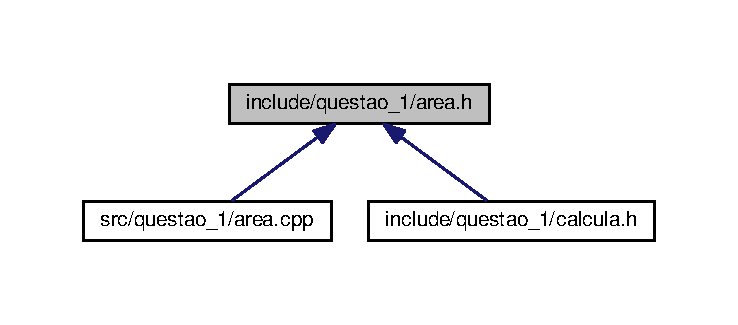
\includegraphics[width=350pt]{area_8h__dep__incl}
\end{center}
\end{figure}
\subsection*{Funções}
\begin{DoxyCompactItemize}
\item 
float \hyperlink{group__Figuras__Planas__CalcArea_gad3dd4559c961d21265a1fe46e7d5c3cc}{triangulo\+Area} (float \&base)
\begin{DoxyCompactList}\small\item\em Função que calcula o valor da área do triangulo. \end{DoxyCompactList}\item 
float \hyperlink{group__Figuras__Planas__CalcArea_gaadec7ea7b857fb93862af9da30f4b896}{retangulo\+Area} (float \&base, float \&altura)
\begin{DoxyCompactList}\small\item\em Função que calcula o valor da área do retângulo. \end{DoxyCompactList}\item 
float \hyperlink{group__Figuras__Planas__CalcArea_gac85a6a6234680349b5b8329d4333567e}{quadrado\+Area} (float \&lado)
\begin{DoxyCompactList}\small\item\em Função que calcula o valor da área do quadrado. \end{DoxyCompactList}\item 
float \hyperlink{group__Figuras__Planas__CalcArea_gac50529a5e8458336df0f0e2329e49833}{circulo\+Area} (float \&raio)
\begin{DoxyCompactList}\small\item\em Função que calcula o valor da área do círculo. \end{DoxyCompactList}\item 
float \hyperlink{group__Figuras__Espaciais__CalcArea_ga10226ad45447d70353626a01897d1b06}{area\+Piramide} (float \&base, float \&altura)
\begin{DoxyCompactList}\small\item\em Função que calcula o valor da área da pirâmide. \end{DoxyCompactList}\item 
float \hyperlink{group__Figuras__Espaciais__CalcArea_gab519a0d997044a93085abaaaf6270ab5}{area\+Cubo} (float \&aresta)
\begin{DoxyCompactList}\small\item\em Função que calcula o valor da área do cubo. \end{DoxyCompactList}\item 
float \hyperlink{group__Figuras__Espaciais__CalcArea_gaff7dfecfa742b07c8e8e243325d95117}{area\+Paralelepipedo} (float \&aresta1, float \&aresta2, float \&aresta3)
\begin{DoxyCompactList}\small\item\em Função que calcula o valor da área do paralelepípedo. \end{DoxyCompactList}\item 
float \hyperlink{group__Figuras__Espaciais__CalcArea_ga2d0b18f7e5391dd6a8bff93bb679171a}{area\+Esfera} (float \&raio)
\begin{DoxyCompactList}\small\item\em Função que calcula o valor da área da esfera. \end{DoxyCompactList}\end{DoxyCompactItemize}


\subsection{Descrição Detalhada}
Arquivo cabeçalho contendo a definicao das funções que calculam a área das figuras geométricas. 

\begin{DoxyAuthor}{Autor}
Ariel Oliveira (\href{mailto:ariel.oliveira01@gmail.com}{\tt ariel.\+oliveira01@gmail.\+com}) 
\end{DoxyAuthor}
\begin{DoxySince}{Desde}
10/08/2017 
\end{DoxySince}
\begin{DoxyDate}{Data}
15/08/2017 
\end{DoxyDate}

\hypertarget{calcula_8h}{}\section{Referência do Arquivo include/questao\+\_\+1/calcula.h}
\label{calcula_8h}\index{include/questao\+\_\+1/calcula.\+h@{include/questao\+\_\+1/calcula.\+h}}


Arquivo cabeçalho contendo a definição das funções que solicitam ao usuário os dados necessários para o cálculo da área, perímetroe volume com a figura geométrica e chamam as funções que realizam essa operação.  


{\ttfamily \#include \char`\"{}area.\+h\char`\"{}}\\*
{\ttfamily \#include \char`\"{}perimetro.\+h\char`\"{}}\\*
{\ttfamily \#include \char`\"{}volume.\+h\char`\"{}}\\*
Gráfico de dependência de inclusões para calcula.\+h\+:
\nopagebreak
\begin{figure}[H]
\begin{center}
\leavevmode
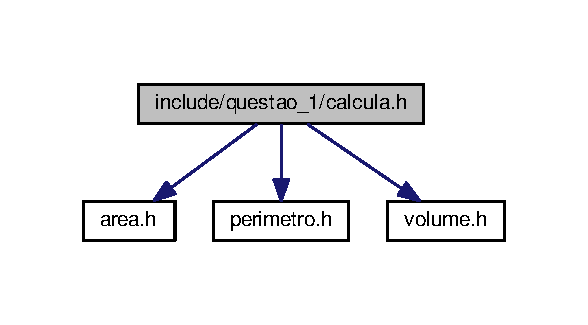
\includegraphics[width=282pt]{calcula_8h__incl}
\end{center}
\end{figure}
\subsection*{Funções}
\begin{DoxyCompactItemize}
\item 
void \hyperlink{group__Figuras__Planas__Imprime__Area_gac0d6d9fb68ed0e43ad9780f0c86cac51}{calc\+Area\+Triangulo} (float \&base)
\begin{DoxyCompactList}\small\item\em Função que imprime o valor da área do triângulo. \end{DoxyCompactList}\item 
void \hyperlink{group__Figuras__Planas__Imprime__Area_ga1091311f26d5adb888dae930fc1ec7d6}{calc\+Area\+Retangulo} (float \&base, float \&altura)
\begin{DoxyCompactList}\small\item\em Função que imprime o valor da área do retângulo. \end{DoxyCompactList}\item 
void \hyperlink{group__Figuras__Planas__Imprime__Area_gaabb19ec0d92baa5524a15b463f854158}{calc\+Area\+Quadrado} (float \&base)
\begin{DoxyCompactList}\small\item\em Função que imprime o valor da área do quadrado. \end{DoxyCompactList}\item 
void \hyperlink{group__Figuras__Planas__Imprime__Area_gafc4965f40035f915dd29f3a2fe680339}{calc\+Area\+Circulo} (float \&raio)
\begin{DoxyCompactList}\small\item\em Função que imprime o valor da área do círculo. \end{DoxyCompactList}\item 
void \hyperlink{group__Figuras__Espaciais__Imprime__Area_gae484b707bcee07b0c5580440923326aa}{calc\+Area\+Piramide} (float \&base, float \&altura)
\begin{DoxyCompactList}\small\item\em Função que imprime o valor da área da pirâmide. \end{DoxyCompactList}\item 
void \hyperlink{group__Figuras__Espaciais__Imprime__Area_ga54aa7364c2caf59fa3d1b1b303901050}{calc\+Area\+Cubo} (float \&aresta)
\begin{DoxyCompactList}\small\item\em Função que imprime o valor da área do círculo. \end{DoxyCompactList}\item 
void \hyperlink{group__Figuras__Espaciais__Imprime__Area_ga153e7a3b91362f17f7f22919dde85ebc}{calc\+Area\+Paralelepipedo} (float \&aresta1, float \&aresta2, float \&aresta3)
\begin{DoxyCompactList}\small\item\em Função que imprime o valor da área do paralelepípedo. \end{DoxyCompactList}\item 
void \hyperlink{group__Figuras__Espaciais__Imprime__Area_ga3a49e8821532ada5f803c815f8d99825}{calc\+Area\+Esfera} (float \&raio)
\begin{DoxyCompactList}\small\item\em Função que imprime o valor da área do círculo. \end{DoxyCompactList}\item 
void \hyperlink{group__Figuras__Planas__Imprime__Perimetro_gae49d939eed738e7168cd0efd8b40c09c}{calc\+Perimetro\+Triangulo} (float \&base)
\begin{DoxyCompactList}\small\item\em Funcao que imprime o valor do perimetro do triangulo. \end{DoxyCompactList}\item 
void \hyperlink{group__Figuras__Planas__Imprime__Perimetro_gab29565d71c21097aef26e73d36b9c8a6}{calc\+Perimetro\+Retangulo} (float \&base, float \&altura)
\begin{DoxyCompactList}\small\item\em Funcao que imprime o valor do perimetro do retangulo. \end{DoxyCompactList}\item 
void \hyperlink{group__Figuras__Planas__Imprime__Perimetro_gacaef8cc731e8f6564e033dadcbefa04f}{calc\+Perimetro\+Quadrado} (float \&base)
\begin{DoxyCompactList}\small\item\em Funcao que imprime o valor do perimetro do quadrado. \end{DoxyCompactList}\item 
void \hyperlink{group__Figuras__Planas__Imprime__Perimetro_ga6f116584d476bf2a78f83cb668e1f25b}{calc\+Perimetro\+Circulo} (float \&raio)
\begin{DoxyCompactList}\small\item\em Funcao que imprime o valor do perimetro do circulo. \end{DoxyCompactList}\item 
void \hyperlink{group__Figuras__Espaciais__Imprime__Volume_gaa5acf0ff0f4eb8061d1b86334d2838de}{calc\+Volume\+Piramide} (float \&base, float \&altura)
\begin{DoxyCompactList}\small\item\em Função que imprime o valor do volume da pirâmide. \end{DoxyCompactList}\item 
void \hyperlink{group__Figuras__Espaciais__Imprime__Volume_gaf35d29634faa808e187b6635ac6e1fb9}{calc\+Volume\+Cubo} (float \&aresta)
\begin{DoxyCompactList}\small\item\em Função que imprime o valor do volume do cubo. \end{DoxyCompactList}\item 
void \hyperlink{group__Figuras__Espaciais__Imprime__Volume_ga994d3c26012b734a4cbabf0ce0c7b75b}{calc\+Volume\+Paralelepipedo} (float \&aresta1, float \&aresta2, float \&aresta3)
\begin{DoxyCompactList}\small\item\em Função que imprime o valor do volume do paralelepípedo. \end{DoxyCompactList}\item 
void \hyperlink{group__Figuras__Espaciais__Imprime__Volume_gaddef3fdcde1a2b12007610961caffae5}{calc\+Volume\+Esfera} (float \&raio)
\begin{DoxyCompactList}\small\item\em Função que imprime o valor do volume da esfera. \end{DoxyCompactList}\end{DoxyCompactItemize}


\subsection{Descrição Detalhada}
Arquivo cabeçalho contendo a definição das funções que solicitam ao usuário os dados necessários para o cálculo da área, perímetroe volume com a figura geométrica e chamam as funções que realizam essa operação. 

\begin{DoxyAuthor}{Autor}
Ariel Oliveira (\href{mailto:ariel.oliveira01@gmail.com}{\tt ariel.\+oliveira01@gmail.\+com}) 
\end{DoxyAuthor}
\begin{DoxySince}{Desde}
10/08/2017 
\end{DoxySince}
\begin{DoxyDate}{Data}
15/08/2017 
\end{DoxyDate}
\begin{DoxySeeAlso}{Veja também}
\hyperlink{area_8h}{area.\+h} 
\end{DoxySeeAlso}

\hypertarget{perimetro_8h}{}\section{include/perimetro.h File Reference}
\label{perimetro_8h}\index{include/perimetro.\+h@{include/perimetro.\+h}}


Arquivo cabeçalho contendo a definição das funções que calculam o perímetro de figuras geométricas planas.  


This graph shows which files directly or indirectly include this file\+:
\nopagebreak
\begin{figure}[H]
\begin{center}
\leavevmode
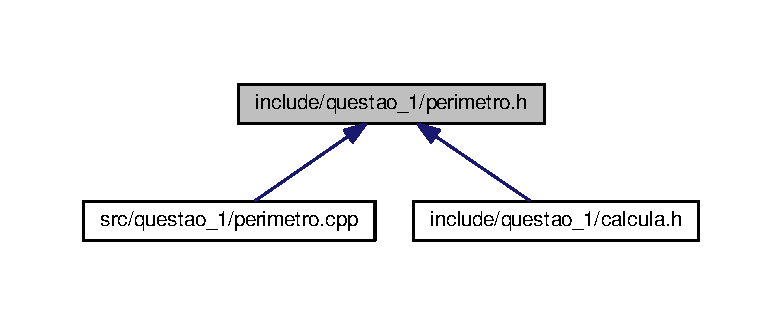
\includegraphics[width=341pt]{perimetro_8h__dep__incl}
\end{center}
\end{figure}
\subsection*{Functions}
\begin{DoxyCompactItemize}
\item 
float \hyperlink{group__Calc__Perimetro_ga76a18caf86cad87741930b6b73a28e6d}{triangulo\+Perimetro} (float \&base)
\begin{DoxyCompactList}\small\item\em Função que calcula o valor do perímetro do triângulo. \end{DoxyCompactList}\item 
float \hyperlink{group__Calc__Perimetro_ga818dc286a8e9892293bddf8c2c4611dd}{retangulo\+Perimetro} (float \&base, float \&altura)
\begin{DoxyCompactList}\small\item\em Função que calcula o valor do perímetro do retângulo. \end{DoxyCompactList}\item 
float \hyperlink{group__Calc__Perimetro_ga262504d9854cd41bc2519504de0531ca}{quadrado\+Perimetro} (float \&base)
\begin{DoxyCompactList}\small\item\em Função que calcula o valor do perímetro do quadrado. \end{DoxyCompactList}\item 
float \hyperlink{group__Calc__Perimetro_gabf774992f344a535b77e941cabb7e2f0}{circulo\+Perimetro} (float \&raio)
\begin{DoxyCompactList}\small\item\em Função que calcula o valor do perímetro do círculo. \end{DoxyCompactList}\end{DoxyCompactItemize}


\subsection{Detailed Description}
Arquivo cabeçalho contendo a definição das funções que calculam o perímetro de figuras geométricas planas. 

\begin{DoxyAuthor}{Author}
Gabriel Barbosa (\href{mailto:gbsbarbosa.gb@gmail.com}{\tt gbsbarbosa.\+gb@gmail.\+com}) 

Ariel Oliveira (\href{mailto:ariel.oliveira01@gmail.com}{\tt ariel.\+oliveira01@gmail.\+com}) 
\end{DoxyAuthor}
\begin{DoxySince}{Since}
12/03/2017 
\end{DoxySince}
\begin{DoxyDate}{Date}
21/03/2017 
\end{DoxyDate}

\hypertarget{volume_8h}{}\section{Referência do Arquivo include/questao\+\_\+1/volume.h}
\label{volume_8h}\index{include/questao\+\_\+1/volume.\+h@{include/questao\+\_\+1/volume.\+h}}


Arquivo cabeçalho contendo a definição das funções que calculam o volume de figuras geométricas espaciais.  


Este grafo mostra quais arquivos estão direta ou indiretamente relacionados com este arquivo\+:
\nopagebreak
\begin{figure}[H]
\begin{center}
\leavevmode
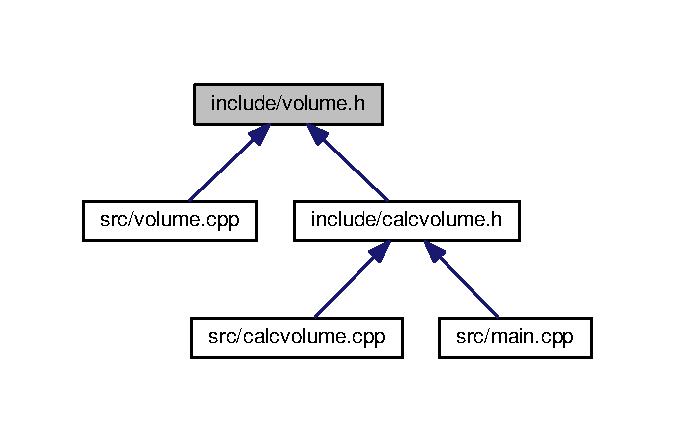
\includegraphics[width=350pt]{volume_8h__dep__incl}
\end{center}
\end{figure}
\subsection*{Funções}
\begin{DoxyCompactItemize}
\item 
float \hyperlink{group__Calc__Volume_ga4a36098bad980501fa8e5d0229309098}{volume\+Piramide} (float \&base, float \&altura)
\begin{DoxyCompactList}\small\item\em Função que calcula o valor do volume da pirâmide. \end{DoxyCompactList}\item 
float \hyperlink{group__Calc__Volume_ga43aaef1a010e2ccbe7e5389aa5be3366}{volume\+Cubo} (float \&aresta)
\begin{DoxyCompactList}\small\item\em Função que calcula o valor do volume do cubo. \end{DoxyCompactList}\item 
float \hyperlink{group__Calc__Volume_gadf67b3277ecfcf3e6e225e1f66e30a23}{volume\+Paralelepipedo} (float \&aresta1, float \&aresta2, float \&aresta3)
\begin{DoxyCompactList}\small\item\em Função que calcula o valor do volume do paralelepípedo. \end{DoxyCompactList}\item 
float \hyperlink{group__Calc__Volume_gaf649387c42d43094c7c81e2f26face42}{volume\+Esfera} (float \&raio)
\begin{DoxyCompactList}\small\item\em Função que calcula o valor do volume da esfera. \end{DoxyCompactList}\end{DoxyCompactItemize}


\subsection{Descrição Detalhada}
Arquivo cabeçalho contendo a definição das funções que calculam o volume de figuras geométricas espaciais. 

\begin{DoxyAuthor}{Autor}
Ariel Oliveira (\href{mailto:ariel.oliveira01@gmail.com}{\tt ariel.\+oliveira01@gmail.\+com}) 
\end{DoxyAuthor}
\begin{DoxySince}{Desde}
10/08/2017 
\end{DoxySince}
\begin{DoxyDate}{Data}
15/08/2017 
\end{DoxyDate}

\hypertarget{fatorial_8h}{}\section{Referência do Arquivo include/questao\+\_\+2/fatorial.h}
\label{fatorial_8h}\index{include/questao\+\_\+2/fatorial.\+h@{include/questao\+\_\+2/fatorial.\+h}}


Arquivo cabeçalho contendo a definicao das funções que calculam o fatorial do número inteiro inserido pelo usuário.  


Este grafo mostra quais arquivos estão direta ou indiretamente relacionados com este arquivo\+:
\nopagebreak
\begin{figure}[H]
\begin{center}
\leavevmode
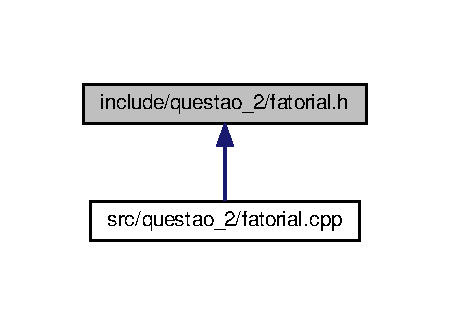
\includegraphics[width=216pt]{fatorial_8h__dep__incl}
\end{center}
\end{figure}
\subsection*{Funções}
\begin{DoxyCompactItemize}
\item 
int \hyperlink{fatorial_8h_aec81b918c463533840b372d476838d1a}{fatorial} (int n)
\begin{DoxyCompactList}\small\item\em Função que calcula o fatorial de um dado número. \end{DoxyCompactList}\end{DoxyCompactItemize}


\subsection{Descrição Detalhada}
Arquivo cabeçalho contendo a definicao das funções que calculam o fatorial do número inteiro inserido pelo usuário. 

\begin{DoxyAuthor}{Autor}
Ariel Oliveira (\href{mailto:ariel.oliveira01@gmail.com}{\tt ariel.\+oliveira01@gmail.\+com}) 
\end{DoxyAuthor}
\begin{DoxySince}{Desde}
10/08/2017 
\end{DoxySince}
\begin{DoxyDate}{Data}
15/08/2017 
\end{DoxyDate}


\subsection{Funções}
\index{fatorial.\+h@{fatorial.\+h}!fatorial@{fatorial}}
\index{fatorial@{fatorial}!fatorial.\+h@{fatorial.\+h}}
\subsubsection[{\texorpdfstring{fatorial(int n)}{fatorial(int n)}}]{\setlength{\rightskip}{0pt plus 5cm}int fatorial (
\begin{DoxyParamCaption}
\item[{int}]{n}
\end{DoxyParamCaption}
)}\hypertarget{fatorial_8h_aec81b918c463533840b372d476838d1a}{}\label{fatorial_8h_aec81b918c463533840b372d476838d1a}


Função que calcula o fatorial de um dado número. 


\begin{DoxyParams}{Parâmetros}
{\em n} & N inteiro a ser calculado \\
\hline
\end{DoxyParams}

\hypertarget{primalidade_8h}{}\section{Referência do Arquivo include/questao\+\_\+2/primalidade.h}
\label{primalidade_8h}\index{include/questao\+\_\+2/primalidade.\+h@{include/questao\+\_\+2/primalidade.\+h}}


Arquivo cabeçalho contendo a definicao da função recursiva que calcula o maior número primo anterior a um determinado inteiro.  


{\ttfamily \#include $<$math.\+h$>$}\\*
Gráfico de dependência de inclusões para primalidade.\+h\+:
\nopagebreak
\begin{figure}[H]
\begin{center}
\leavevmode
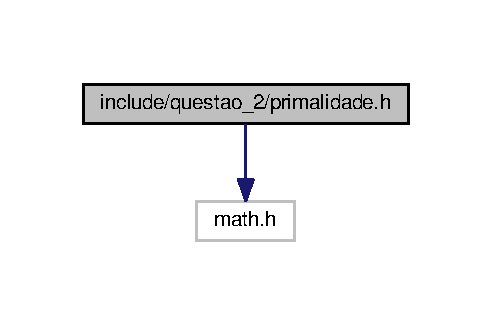
\includegraphics[width=236pt]{primalidade_8h__incl}
\end{center}
\end{figure}
Este grafo mostra quais arquivos estão direta ou indiretamente relacionados com este arquivo\+:
\nopagebreak
\begin{figure}[H]
\begin{center}
\leavevmode
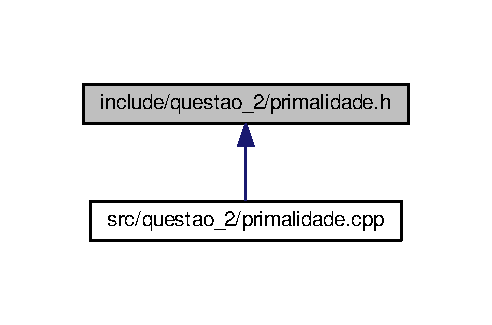
\includegraphics[width=236pt]{primalidade_8h__dep__incl}
\end{center}
\end{figure}
\subsection*{Funções}
\begin{DoxyCompactItemize}
\item 
int \hyperlink{primalidade_8h_ac5bda7b7f8ca82ed9f53d0cb71bef1c1}{maior\+Primo} (int n, int k)
\begin{DoxyCompactList}\small\item\em Função que calcula o fatorial de um dado número. \end{DoxyCompactList}\end{DoxyCompactItemize}


\subsection{Descrição Detalhada}
Arquivo cabeçalho contendo a definicao da função recursiva que calcula o maior número primo anterior a um determinado inteiro. 

\begin{DoxyAuthor}{Autor}
Ariel Oliveira (\href{mailto:ariel.oliveira01@gmail.com}{\tt ariel.\+oliveira01@gmail.\+com}) 
\end{DoxyAuthor}
\begin{DoxySince}{Desde}
10/08/2017 
\end{DoxySince}
\begin{DoxyDate}{Data}
15/08/2017 
\end{DoxyDate}


\subsection{Funções}
\index{primalidade.\+h@{primalidade.\+h}!maior\+Primo@{maior\+Primo}}
\index{maior\+Primo@{maior\+Primo}!primalidade.\+h@{primalidade.\+h}}
\subsubsection[{\texorpdfstring{maior\+Primo(int n, int k)}{maiorPrimo(int n, int k)}}]{\setlength{\rightskip}{0pt plus 5cm}int maior\+Primo (
\begin{DoxyParamCaption}
\item[{int}]{n, }
\item[{int}]{k}
\end{DoxyParamCaption}
)}\hypertarget{primalidade_8h_ac5bda7b7f8ca82ed9f53d0cb71bef1c1}{}\label{primalidade_8h_ac5bda7b7f8ca82ed9f53d0cb71bef1c1}


Função que calcula o fatorial de um dado número. 


\begin{DoxyParams}{Parâmetros}
{\em n} & N inteiro a ser calculado \\
\hline
\end{DoxyParams}

\hypertarget{area_8cpp}{}\section{src/area.cpp File Reference}
\label{area_8cpp}\index{src/area.\+cpp@{src/area.\+cpp}}


Arquivo cabeçalho contendo a definição das funções que calculam a área das figuras geométricas.  


{\ttfamily \#include $<$cmath$>$}\\*
{\ttfamily \#include \char`\"{}area.\+h\char`\"{}}\\*
Include dependency graph for area.\+cpp\+:
% FIG 0
\subsection*{Macros}
\begin{DoxyCompactItemize}
\item 
\#define {\bfseries PI}~3.\+1415\hypertarget{area_8cpp_a598a3330b3c21701223ee0ca14316eca}{}\label{area_8cpp_a598a3330b3c21701223ee0ca14316eca}

\item 
\#define {\bfseries pitagoras}(a,  b)~(pow(a,2) -\/ pow(b,2))\hypertarget{area_8cpp_a4544bdcd1e3ebe0263d82aad9efa4901}{}\label{area_8cpp_a4544bdcd1e3ebe0263d82aad9efa4901}

\end{DoxyCompactItemize}
\subsection*{Functions}
\begin{DoxyCompactItemize}
\item 
float \hyperlink{area_8cpp_ad3dd4559c961d21265a1fe46e7d5c3cc}{triangulo\+Area} (float \&base)
\begin{DoxyCompactList}\small\item\em Função que calcula o valor da área do triângulo. \end{DoxyCompactList}\item 
float \hyperlink{area_8cpp_aadec7ea7b857fb93862af9da30f4b896}{retangulo\+Area} (float \&base, float \&altura)
\begin{DoxyCompactList}\small\item\em Função que calcula o valor da área do retângulo. \end{DoxyCompactList}\item 
float \hyperlink{area_8cpp_ac85a6a6234680349b5b8329d4333567e}{quadrado\+Area} (float \&lado)
\begin{DoxyCompactList}\small\item\em Função que calcula o valor da área do quadrado. \end{DoxyCompactList}\item 
float \hyperlink{area_8cpp_ac50529a5e8458336df0f0e2329e49833}{circulo\+Area} (float \&raio)
\begin{DoxyCompactList}\small\item\em Função que calcula o valor da área do círculo. \end{DoxyCompactList}\item 
float \hyperlink{area_8cpp_a10226ad45447d70353626a01897d1b06}{area\+Piramide} (float \&base, float \&altura)
\begin{DoxyCompactList}\small\item\em Função que calcula o valor da área da pirâmide. \end{DoxyCompactList}\item 
float \hyperlink{area_8cpp_ab519a0d997044a93085abaaaf6270ab5}{area\+Cubo} (float \&aresta)
\begin{DoxyCompactList}\small\item\em Função que calcula o valor da área do cubo. \end{DoxyCompactList}\item 
float \hyperlink{area_8cpp_aff7dfecfa742b07c8e8e243325d95117}{area\+Paralelepipedo} (float \&aresta1, float \&aresta2, float \&aresta3)
\begin{DoxyCompactList}\small\item\em Função que calcula o valor da área do paralelepípedo. \end{DoxyCompactList}\item 
float \hyperlink{area_8cpp_a2d0b18f7e5391dd6a8bff93bb679171a}{area\+Esfera} (float \&raio)
\begin{DoxyCompactList}\small\item\em Função que calcula o valor da área da esfera. \end{DoxyCompactList}\end{DoxyCompactItemize}


\subsection{Detailed Description}
Arquivo cabeçalho contendo a definição das funções que calculam a área das figuras geométricas. 

\begin{DoxyAuthor}{Author}
Gabriel Barbosa (\href{mailto:gbsbarbosa.gb@gmail.com}{\tt gbsbarbosa.\+gb@gmail.\+com}) 

Ariel Oliveira (\href{mailto:ariel.oliveira01@gmail.com}{\tt ariel.\+oliveira01@gmail.\+com}) 
\end{DoxyAuthor}
\begin{DoxySince}{Since}
09/03/2017 
\end{DoxySince}
\begin{DoxyDate}{Date}
12/03/2017 
\end{DoxyDate}
\begin{DoxySeeAlso}{See also}
\hyperlink{area_8h}{area.\+h} 
\end{DoxySeeAlso}


\subsection{Function Documentation}
\index{area.\+cpp@{area.\+cpp}!area\+Cubo@{area\+Cubo}}
\index{area\+Cubo@{area\+Cubo}!area.\+cpp@{area.\+cpp}}
\subsubsection[{\texorpdfstring{area\+Cubo(float \&aresta)}{areaCubo(float &aresta)}}]{\setlength{\rightskip}{0pt plus 5cm}float area\+Cubo (
\begin{DoxyParamCaption}
\item[{float \&}]{aresta}
\end{DoxyParamCaption}
)}\hypertarget{area_8cpp_ab519a0d997044a93085abaaaf6270ab5}{}\label{area_8cpp_ab519a0d997044a93085abaaaf6270ab5}


Função que calcula o valor da área do cubo. 


\begin{DoxyParams}{Parameters}
{\em aresta} & A\+R\+E\+S\+TA valor da aresta do cubo \\
\hline
\end{DoxyParams}
\begin{DoxyReturn}{Returns}
área do triângulo 
\end{DoxyReturn}
\index{area.\+cpp@{area.\+cpp}!area\+Esfera@{area\+Esfera}}
\index{area\+Esfera@{area\+Esfera}!area.\+cpp@{area.\+cpp}}
\subsubsection[{\texorpdfstring{area\+Esfera(float \&raio)}{areaEsfera(float &raio)}}]{\setlength{\rightskip}{0pt plus 5cm}float area\+Esfera (
\begin{DoxyParamCaption}
\item[{float \&}]{raio}
\end{DoxyParamCaption}
)}\hypertarget{area_8cpp_a2d0b18f7e5391dd6a8bff93bb679171a}{}\label{area_8cpp_a2d0b18f7e5391dd6a8bff93bb679171a}


Função que calcula o valor da área da esfera. 


\begin{DoxyParams}{Parameters}
{\em raio} & R\+A\+IO valor do raio da esfera \\
\hline
\end{DoxyParams}
\begin{DoxyReturn}{Returns}
área da esfera 
\end{DoxyReturn}
\index{area.\+cpp@{area.\+cpp}!area\+Paralelepipedo@{area\+Paralelepipedo}}
\index{area\+Paralelepipedo@{area\+Paralelepipedo}!area.\+cpp@{area.\+cpp}}
\subsubsection[{\texorpdfstring{area\+Paralelepipedo(float \&aresta1, float \&aresta2, float \&aresta3)}{areaParalelepipedo(float &aresta1, float &aresta2, float &aresta3)}}]{\setlength{\rightskip}{0pt plus 5cm}float area\+Paralelepipedo (
\begin{DoxyParamCaption}
\item[{float \&}]{aresta1, }
\item[{float \&}]{aresta2, }
\item[{float \&}]{aresta3}
\end{DoxyParamCaption}
)}\hypertarget{area_8cpp_aff7dfecfa742b07c8e8e243325d95117}{}\label{area_8cpp_aff7dfecfa742b07c8e8e243325d95117}


Função que calcula o valor da área do paralelepípedo. 


\begin{DoxyParams}{Parameters}
{\em aresta1} & A\+R\+E\+S\+T\+A1 valor da aresta \#1 do paralelepípedo \\
\hline
{\em aresta2} & A\+R\+E\+S\+T\+A2 valor da aresta \#2 do paralelepípedo \\
\hline
{\em aresta3} & A\+R\+E\+S\+T\+A3 valor da aresta \#3 do paralelepípedo \\
\hline
\end{DoxyParams}
\begin{DoxyReturn}{Returns}
área do paralelepípedo 
\end{DoxyReturn}
\index{area.\+cpp@{area.\+cpp}!area\+Piramide@{area\+Piramide}}
\index{area\+Piramide@{area\+Piramide}!area.\+cpp@{area.\+cpp}}
\subsubsection[{\texorpdfstring{area\+Piramide(float \&base, float \&altura)}{areaPiramide(float &base, float &altura)}}]{\setlength{\rightskip}{0pt plus 5cm}float area\+Piramide (
\begin{DoxyParamCaption}
\item[{float \&}]{base, }
\item[{float \&}]{altura}
\end{DoxyParamCaption}
)}\hypertarget{area_8cpp_a10226ad45447d70353626a01897d1b06}{}\label{area_8cpp_a10226ad45447d70353626a01897d1b06}


Função que calcula o valor da área da pirâmide. 


\begin{DoxyParams}{Parameters}
{\em base} & B\+A\+SE valor da base da pirâmide \\
\hline
{\em altura} & A\+L\+T\+U\+RA valor da altura da pirâmide \\
\hline
\end{DoxyParams}
\begin{DoxyReturn}{Returns}
área da pirâmide 
\end{DoxyReturn}
\index{area.\+cpp@{area.\+cpp}!circulo\+Area@{circulo\+Area}}
\index{circulo\+Area@{circulo\+Area}!area.\+cpp@{area.\+cpp}}
\subsubsection[{\texorpdfstring{circulo\+Area(float \&raio)}{circuloArea(float &raio)}}]{\setlength{\rightskip}{0pt plus 5cm}float circulo\+Area (
\begin{DoxyParamCaption}
\item[{float \&}]{raio}
\end{DoxyParamCaption}
)}\hypertarget{area_8cpp_ac50529a5e8458336df0f0e2329e49833}{}\label{area_8cpp_ac50529a5e8458336df0f0e2329e49833}


Função que calcula o valor da área do círculo. 


\begin{DoxyParams}{Parameters}
{\em raio} & R\+A\+IO valor do raio do círculo \\
\hline
\end{DoxyParams}
\begin{DoxyReturn}{Returns}
área do círculo 
\end{DoxyReturn}
\index{area.\+cpp@{area.\+cpp}!quadrado\+Area@{quadrado\+Area}}
\index{quadrado\+Area@{quadrado\+Area}!area.\+cpp@{area.\+cpp}}
\subsubsection[{\texorpdfstring{quadrado\+Area(float \&lado)}{quadradoArea(float &lado)}}]{\setlength{\rightskip}{0pt plus 5cm}float quadrado\+Area (
\begin{DoxyParamCaption}
\item[{float \&}]{lado}
\end{DoxyParamCaption}
)}\hypertarget{area_8cpp_ac85a6a6234680349b5b8329d4333567e}{}\label{area_8cpp_ac85a6a6234680349b5b8329d4333567e}


Função que calcula o valor da área do quadrado. 


\begin{DoxyParams}{Parameters}
{\em lado} & L\+A\+DO valor dos lados do quadrado \\
\hline
\end{DoxyParams}
\begin{DoxyReturn}{Returns}
área do quadrado 
\end{DoxyReturn}
\index{area.\+cpp@{area.\+cpp}!retangulo\+Area@{retangulo\+Area}}
\index{retangulo\+Area@{retangulo\+Area}!area.\+cpp@{area.\+cpp}}
\subsubsection[{\texorpdfstring{retangulo\+Area(float \&base, float \&altura)}{retanguloArea(float &base, float &altura)}}]{\setlength{\rightskip}{0pt plus 5cm}float retangulo\+Area (
\begin{DoxyParamCaption}
\item[{float \&}]{base, }
\item[{float \&}]{altura}
\end{DoxyParamCaption}
)}\hypertarget{area_8cpp_aadec7ea7b857fb93862af9da30f4b896}{}\label{area_8cpp_aadec7ea7b857fb93862af9da30f4b896}


Função que calcula o valor da área do retângulo. 


\begin{DoxyParams}{Parameters}
{\em base} & B\+A\+SE valor da base do retângulo \\
\hline
{\em altura} & A\+L\+T\+U\+RA valor da altura do retângulo \\
\hline
\end{DoxyParams}
\begin{DoxyReturn}{Returns}
área do retângulo 
\end{DoxyReturn}
\index{area.\+cpp@{area.\+cpp}!triangulo\+Area@{triangulo\+Area}}
\index{triangulo\+Area@{triangulo\+Area}!area.\+cpp@{area.\+cpp}}
\subsubsection[{\texorpdfstring{triangulo\+Area(float \&base)}{trianguloArea(float &base)}}]{\setlength{\rightskip}{0pt plus 5cm}float triangulo\+Area (
\begin{DoxyParamCaption}
\item[{float \&}]{base}
\end{DoxyParamCaption}
)}\hypertarget{area_8cpp_ad3dd4559c961d21265a1fe46e7d5c3cc}{}\label{area_8cpp_ad3dd4559c961d21265a1fe46e7d5c3cc}


Função que calcula o valor da área do triângulo. 

Função que calcula o valor da área do triangulo.


\begin{DoxyParams}{Parameters}
{\em base} & B\+A\+SE valor da base da triângulo \\
\hline
\end{DoxyParams}
\begin{DoxyReturn}{Returns}
área do triângulo 
\end{DoxyReturn}

\hypertarget{perimetro_8cpp}{}\section{src/perimetro.cpp File Reference}
\label{perimetro_8cpp}\index{src/perimetro.\+cpp@{src/perimetro.\+cpp}}


Arquivo cabeçalho contendo a definição das funções que calculam o perímetro de figuras geométricas planas.  


{\ttfamily \#include \char`\"{}perimetro.\+h\char`\"{}}\\*
Include dependency graph for perimetro.\+cpp\+:
% FIG 0
\subsection*{Macros}
\begin{DoxyCompactItemize}
\item 
\#define {\bfseries PI}~3.\+1415\hypertarget{perimetro_8cpp_a598a3330b3c21701223ee0ca14316eca}{}\label{perimetro_8cpp_a598a3330b3c21701223ee0ca14316eca}

\end{DoxyCompactItemize}
\subsection*{Functions}
\begin{DoxyCompactItemize}
\item 
float \hyperlink{perimetro_8cpp_a76a18caf86cad87741930b6b73a28e6d}{triangulo\+Perimetro} (float \&base)
\begin{DoxyCompactList}\small\item\em Função que calcula o valor do perimetro do triângulo. \end{DoxyCompactList}\item 
float \hyperlink{perimetro_8cpp_a818dc286a8e9892293bddf8c2c4611dd}{retangulo\+Perimetro} (float \&base, float \&altura)
\begin{DoxyCompactList}\small\item\em Função que calcula o valor do perimetro do retângulo. \end{DoxyCompactList}\item 
float \hyperlink{perimetro_8cpp_a262504d9854cd41bc2519504de0531ca}{quadrado\+Perimetro} (float \&base)
\begin{DoxyCompactList}\small\item\em Função que calcula o valor do perímetro do quadrado. \end{DoxyCompactList}\item 
float \hyperlink{perimetro_8cpp_abf774992f344a535b77e941cabb7e2f0}{circulo\+Perimetro} (float \&raio)
\begin{DoxyCompactList}\small\item\em Função que calcula o valor do perimetro do círculo. \end{DoxyCompactList}\end{DoxyCompactItemize}


\subsection{Detailed Description}
Arquivo cabeçalho contendo a definição das funções que calculam o perímetro de figuras geométricas planas. 

\begin{DoxyAuthor}{Author}
Gabriel Barbosa (\href{mailto:gbsbarbosa.gb@gmail.com}{\tt gbsbarbosa.\+gb@gmail.\+com}) 

Ariel Oliveira (\href{mailto:ariel.oliveira01@gmail.com}{\tt ariel.\+oliveira01@gmail.\+com}) 
\end{DoxyAuthor}
\begin{DoxySince}{Since}
12/03/2017 
\end{DoxySince}
\begin{DoxyDate}{Date}
21/03/2017 
\end{DoxyDate}
\begin{DoxySeeAlso}{See also}
\hyperlink{perimetro_8h}{perimetro.\+h} 
\end{DoxySeeAlso}


\subsection{Function Documentation}
\index{perimetro.\+cpp@{perimetro.\+cpp}!circulo\+Perimetro@{circulo\+Perimetro}}
\index{circulo\+Perimetro@{circulo\+Perimetro}!perimetro.\+cpp@{perimetro.\+cpp}}
\subsubsection[{\texorpdfstring{circulo\+Perimetro(float \&raio)}{circuloPerimetro(float &raio)}}]{\setlength{\rightskip}{0pt plus 5cm}float circulo\+Perimetro (
\begin{DoxyParamCaption}
\item[{float \&}]{raio}
\end{DoxyParamCaption}
)}\hypertarget{perimetro_8cpp_abf774992f344a535b77e941cabb7e2f0}{}\label{perimetro_8cpp_abf774992f344a535b77e941cabb7e2f0}


Função que calcula o valor do perimetro do círculo. 

Funcao que calcula o valor do perimetro do circulo.


\begin{DoxyParams}{Parameters}
{\em raio} & R\+A\+IO valor da base do círculo \\
\hline
\end{DoxyParams}
\index{perimetro.\+cpp@{perimetro.\+cpp}!quadrado\+Perimetro@{quadrado\+Perimetro}}
\index{quadrado\+Perimetro@{quadrado\+Perimetro}!perimetro.\+cpp@{perimetro.\+cpp}}
\subsubsection[{\texorpdfstring{quadrado\+Perimetro(float \&base)}{quadradoPerimetro(float &base)}}]{\setlength{\rightskip}{0pt plus 5cm}float quadrado\+Perimetro (
\begin{DoxyParamCaption}
\item[{float \&}]{base}
\end{DoxyParamCaption}
)}\hypertarget{perimetro_8cpp_a262504d9854cd41bc2519504de0531ca}{}\label{perimetro_8cpp_a262504d9854cd41bc2519504de0531ca}


Função que calcula o valor do perímetro do quadrado. 

Funcao que calcula o valor do perimetro do quadrado.


\begin{DoxyParams}{Parameters}
{\em base} & B\+A\+SE valor da base do quadrado \\
\hline
\end{DoxyParams}
\index{perimetro.\+cpp@{perimetro.\+cpp}!retangulo\+Perimetro@{retangulo\+Perimetro}}
\index{retangulo\+Perimetro@{retangulo\+Perimetro}!perimetro.\+cpp@{perimetro.\+cpp}}
\subsubsection[{\texorpdfstring{retangulo\+Perimetro(float \&base, float \&altura)}{retanguloPerimetro(float &base, float &altura)}}]{\setlength{\rightskip}{0pt plus 5cm}float retangulo\+Perimetro (
\begin{DoxyParamCaption}
\item[{float \&}]{base, }
\item[{float \&}]{altura}
\end{DoxyParamCaption}
)}\hypertarget{perimetro_8cpp_a818dc286a8e9892293bddf8c2c4611dd}{}\label{perimetro_8cpp_a818dc286a8e9892293bddf8c2c4611dd}


Função que calcula o valor do perimetro do retângulo. 

Funcao que calcula o valor do perimetro do retangulo.


\begin{DoxyParams}{Parameters}
{\em base} & B\+A\+SE valor da base do retângulo \\
\hline
{\em altura} & A\+L\+T\+U\+RA valor da altura do retângulo \\
\hline
\end{DoxyParams}
\index{perimetro.\+cpp@{perimetro.\+cpp}!triangulo\+Perimetro@{triangulo\+Perimetro}}
\index{triangulo\+Perimetro@{triangulo\+Perimetro}!perimetro.\+cpp@{perimetro.\+cpp}}
\subsubsection[{\texorpdfstring{triangulo\+Perimetro(float \&base)}{trianguloPerimetro(float &base)}}]{\setlength{\rightskip}{0pt plus 5cm}float triangulo\+Perimetro (
\begin{DoxyParamCaption}
\item[{float \&}]{base}
\end{DoxyParamCaption}
)}\hypertarget{perimetro_8cpp_a76a18caf86cad87741930b6b73a28e6d}{}\label{perimetro_8cpp_a76a18caf86cad87741930b6b73a28e6d}


Função que calcula o valor do perimetro do triângulo. 

Função que calcula o valor do perimetro do triangulo.


\begin{DoxyParams}{Parameters}
{\em base} & B\+A\+SE valor da base do triangulo \\
\hline
\end{DoxyParams}

\hypertarget{volume_8cpp}{}\section{src/volume.cpp File Reference}
\label{volume_8cpp}\index{src/volume.\+cpp@{src/volume.\+cpp}}


Arquivo corpo contendo a Implementação das funções que calculam o volume de figuras geométricas espaciais.  


{\ttfamily \#include $<$cmath$>$}\\*
{\ttfamily \#include \char`\"{}volume.\+h\char`\"{}}\\*
Include dependency graph for volume.\+cpp\+:
\nopagebreak
\begin{figure}[H]
\begin{center}
\leavevmode
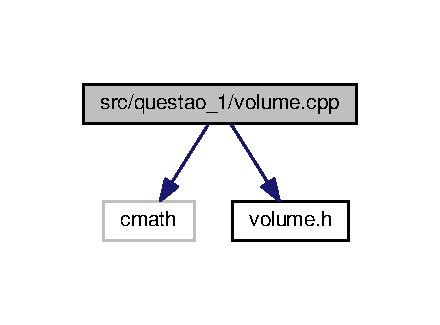
\includegraphics[width=198pt]{volume_8cpp__incl}
\end{center}
\end{figure}
\subsection*{Macros}
\begin{DoxyCompactItemize}
\item 
\#define {\bfseries PI}~3.\+1415\hypertarget{volume_8cpp_a598a3330b3c21701223ee0ca14316eca}{}\label{volume_8cpp_a598a3330b3c21701223ee0ca14316eca}

\end{DoxyCompactItemize}
\subsection*{Functions}
\begin{DoxyCompactItemize}
\item 
float \hyperlink{volume_8cpp_a4a36098bad980501fa8e5d0229309098}{volume\+Piramide} (float \&base, float \&altura)
\begin{DoxyCompactList}\small\item\em Funcao que calcula o valor do volume da piramide. \end{DoxyCompactList}\item 
float \hyperlink{volume_8cpp_a43aaef1a010e2ccbe7e5389aa5be3366}{volume\+Cubo} (float \&aresta)
\begin{DoxyCompactList}\small\item\em Funcao que calcula o valor do volume do cubo. \end{DoxyCompactList}\item 
float \hyperlink{volume_8cpp_adf67b3277ecfcf3e6e225e1f66e30a23}{volume\+Paralelepipedo} (float \&aresta1, float \&aresta2, float \&aresta3)
\begin{DoxyCompactList}\small\item\em Funcao que calcula o valor do volume do paralelepipedo. \end{DoxyCompactList}\item 
float \hyperlink{volume_8cpp_af649387c42d43094c7c81e2f26face42}{volume\+Esfera} (float \&raio)
\begin{DoxyCompactList}\small\item\em Funcao que calcula o valor do volume da esfera. \end{DoxyCompactList}\end{DoxyCompactItemize}


\subsection{Detailed Description}
Arquivo corpo contendo a Implementação das funções que calculam o volume de figuras geométricas espaciais. 

\begin{DoxyAuthor}{Author}
Gabriel Barbosa (\href{mailto:gbsbarbosa.gb@gmail.com}{\tt gbsbarbosa.\+gb@gmail.\+com}) 

Ariel Oliveira (\href{mailto:ariel.oliveira01@gmail.com}{\tt ariel.\+oliveira01@gmail.\+com}) 
\end{DoxyAuthor}
\begin{DoxySince}{Since}
09/03/2017 
\end{DoxySince}
\begin{DoxyDate}{Date}
12/03/2017 
\end{DoxyDate}
\begin{DoxySeeAlso}{See also}
\hyperlink{volume_8h}{volume.\+h} 
\end{DoxySeeAlso}


\subsection{Function Documentation}
\index{volume.\+cpp@{volume.\+cpp}!volume\+Cubo@{volume\+Cubo}}
\index{volume\+Cubo@{volume\+Cubo}!volume.\+cpp@{volume.\+cpp}}
\subsubsection[{\texorpdfstring{volume\+Cubo(float \&aresta)}{volumeCubo(float &aresta)}}]{\setlength{\rightskip}{0pt plus 5cm}float volume\+Cubo (
\begin{DoxyParamCaption}
\item[{float \&}]{aresta}
\end{DoxyParamCaption}
)}\hypertarget{volume_8cpp_a43aaef1a010e2ccbe7e5389aa5be3366}{}\label{volume_8cpp_a43aaef1a010e2ccbe7e5389aa5be3366}


Funcao que calcula o valor do volume do cubo. 


\begin{DoxyParams}{Parameters}
{\em aresta} & A\+R\+E\+S\+TA valor da aresta do cubo \\
\hline
\end{DoxyParams}
\begin{DoxyReturn}{Returns}
Volume do cubo 
\end{DoxyReturn}
\index{volume.\+cpp@{volume.\+cpp}!volume\+Esfera@{volume\+Esfera}}
\index{volume\+Esfera@{volume\+Esfera}!volume.\+cpp@{volume.\+cpp}}
\subsubsection[{\texorpdfstring{volume\+Esfera(float \&raio)}{volumeEsfera(float &raio)}}]{\setlength{\rightskip}{0pt plus 5cm}float volume\+Esfera (
\begin{DoxyParamCaption}
\item[{float \&}]{raio}
\end{DoxyParamCaption}
)}\hypertarget{volume_8cpp_af649387c42d43094c7c81e2f26face42}{}\label{volume_8cpp_af649387c42d43094c7c81e2f26face42}


Funcao que calcula o valor do volume da esfera. 


\begin{DoxyParams}{Parameters}
{\em raio} & R\+A\+IO valor do raio do cubo \\
\hline
\end{DoxyParams}
\begin{DoxyReturn}{Returns}
Volume da esfera 
\end{DoxyReturn}
\index{volume.\+cpp@{volume.\+cpp}!volume\+Paralelepipedo@{volume\+Paralelepipedo}}
\index{volume\+Paralelepipedo@{volume\+Paralelepipedo}!volume.\+cpp@{volume.\+cpp}}
\subsubsection[{\texorpdfstring{volume\+Paralelepipedo(float \&aresta1, float \&aresta2, float \&aresta3)}{volumeParalelepipedo(float &aresta1, float &aresta2, float &aresta3)}}]{\setlength{\rightskip}{0pt plus 5cm}float volume\+Paralelepipedo (
\begin{DoxyParamCaption}
\item[{float \&}]{aresta1, }
\item[{float \&}]{aresta2, }
\item[{float \&}]{aresta3}
\end{DoxyParamCaption}
)}\hypertarget{volume_8cpp_adf67b3277ecfcf3e6e225e1f66e30a23}{}\label{volume_8cpp_adf67b3277ecfcf3e6e225e1f66e30a23}


Funcao que calcula o valor do volume do paralelepipedo. 


\begin{DoxyParams}{Parameters}
{\em aresta1} & A\+R\+E\+S\+T\+A1 valor da aresta \#1 do paralelepipedo \\
\hline
{\em aresta2} & A\+R\+E\+S\+T\+A2 valor da aresta \#2 do paralelepipedo \\
\hline
{\em aresta3} & A\+R\+E\+S\+T\+A3 valor da aresta \#3 do paralelepipedo \\
\hline
\end{DoxyParams}
\begin{DoxyReturn}{Returns}
Valor do volume do paralelepipedo 
\end{DoxyReturn}
\index{volume.\+cpp@{volume.\+cpp}!volume\+Piramide@{volume\+Piramide}}
\index{volume\+Piramide@{volume\+Piramide}!volume.\+cpp@{volume.\+cpp}}
\subsubsection[{\texorpdfstring{volume\+Piramide(float \&base, float \&altura)}{volumePiramide(float &base, float &altura)}}]{\setlength{\rightskip}{0pt plus 5cm}float volume\+Piramide (
\begin{DoxyParamCaption}
\item[{float \&}]{base, }
\item[{float \&}]{altura}
\end{DoxyParamCaption}
)}\hypertarget{volume_8cpp_a4a36098bad980501fa8e5d0229309098}{}\label{volume_8cpp_a4a36098bad980501fa8e5d0229309098}


Funcao que calcula o valor do volume da piramide. 

Função que calcula o valor do volume da pirâmide.


\begin{DoxyParams}{Parameters}
{\em base} & B\+A\+SE valor da base da piramide \\
\hline
{\em altura} & A\+L\+T\+U\+RA valor da altura da piramide \\
\hline
\end{DoxyParams}
\begin{DoxyReturn}{Returns}
Volume da piramide 
\end{DoxyReturn}

\hypertarget{fatorial_8cpp}{}\section{Referência do Arquivo src/questao\+\_\+2/fatorial.cpp}
\label{fatorial_8cpp}\index{src/questao\+\_\+2/fatorial.\+cpp@{src/questao\+\_\+2/fatorial.\+cpp}}


Arquivo contendo a implementação da função que calcula o fatorial do número inteiro inserido pelo usuário.  


{\ttfamily \#include \char`\"{}fatorial.\+h\char`\"{}}\\*
Gráfico de dependência de inclusões para fatorial.\+cpp\+:
\nopagebreak
\begin{figure}[H]
\begin{center}
\leavevmode
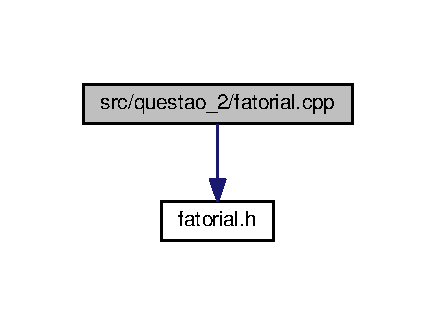
\includegraphics[width=209pt]{fatorial_8cpp__incl}
\end{center}
\end{figure}
\subsection*{Funções}
\begin{DoxyCompactItemize}
\item 
int \hyperlink{fatorial_8cpp_aec81b918c463533840b372d476838d1a}{fatorial} (int n)
\begin{DoxyCompactList}\small\item\em Função que calcula o fatorial de um dado número. \end{DoxyCompactList}\end{DoxyCompactItemize}


\subsection{Descrição Detalhada}
Arquivo contendo a implementação da função que calcula o fatorial do número inteiro inserido pelo usuário. 

\begin{DoxyAuthor}{Autor}
Ariel Oliveira (\href{mailto:ariel.oliveira01@gmail.com}{\tt ariel.\+oliveira01@gmail.\+com}) 
\end{DoxyAuthor}
\begin{DoxySince}{Desde}
10/08/2017 
\end{DoxySince}
\begin{DoxyDate}{Data}
15/08/2017 
\end{DoxyDate}


\subsection{Funções}
\index{fatorial.\+cpp@{fatorial.\+cpp}!fatorial@{fatorial}}
\index{fatorial@{fatorial}!fatorial.\+cpp@{fatorial.\+cpp}}
\subsubsection[{\texorpdfstring{fatorial(int n)}{fatorial(int n)}}]{\setlength{\rightskip}{0pt plus 5cm}int fatorial (
\begin{DoxyParamCaption}
\item[{int}]{n}
\end{DoxyParamCaption}
)}\hypertarget{fatorial_8cpp_aec81b918c463533840b372d476838d1a}{}\label{fatorial_8cpp_aec81b918c463533840b372d476838d1a}


Função que calcula o fatorial de um dado número. 


\begin{DoxyParams}{Parâmetros}
{\em n} & N inteiro a ser calculado \\
\hline
\end{DoxyParams}

\hypertarget{primalidade_8cpp}{}\section{Referência do Arquivo src/questao\+\_\+2/primalidade.cpp}
\label{primalidade_8cpp}\index{src/questao\+\_\+2/primalidade.\+cpp@{src/questao\+\_\+2/primalidade.\+cpp}}


Arquivo corpo contendo a implementação da função recursiva que calcula o maior número primo anterior a um determinado inteiro.  


{\ttfamily \#include \char`\"{}primalidade.\+h\char`\"{}}\\*
Gráfico de dependência de inclusões para primalidade.\+cpp\+:
\nopagebreak
\begin{figure}[H]
\begin{center}
\leavevmode
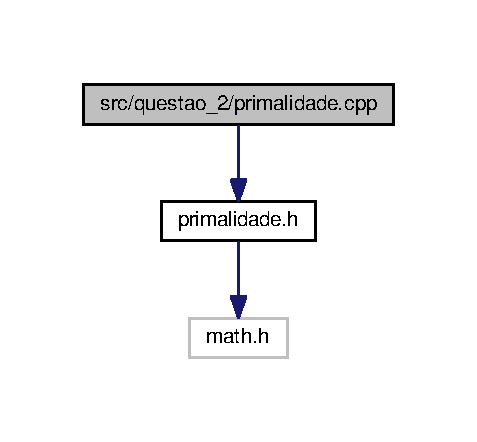
\includegraphics[width=229pt]{primalidade_8cpp__incl}
\end{center}
\end{figure}
\subsection*{Funções}
\begin{DoxyCompactItemize}
\item 
int \hyperlink{primalidade_8cpp_ac5bda7b7f8ca82ed9f53d0cb71bef1c1}{maior\+Primo} (int n, int k)
\begin{DoxyCompactList}\small\item\em Função que calcula o fatorial de um dado número. \end{DoxyCompactList}\end{DoxyCompactItemize}


\subsection{Descrição Detalhada}
Arquivo corpo contendo a implementação da função recursiva que calcula o maior número primo anterior a um determinado inteiro. 

\begin{DoxyAuthor}{Autor}
Ariel Oliveira (\href{mailto:ariel.oliveira01@gmail.com}{\tt ariel.\+oliveira01@gmail.\+com}) 
\end{DoxyAuthor}
\begin{DoxySince}{Desde}
10/08/2017 
\end{DoxySince}
\begin{DoxyDate}{Data}
15/08/2017 
\end{DoxyDate}


\subsection{Funções}
\index{primalidade.\+cpp@{primalidade.\+cpp}!maior\+Primo@{maior\+Primo}}
\index{maior\+Primo@{maior\+Primo}!primalidade.\+cpp@{primalidade.\+cpp}}
\subsubsection[{\texorpdfstring{maior\+Primo(int n, int k)}{maiorPrimo(int n, int k)}}]{\setlength{\rightskip}{0pt plus 5cm}int maior\+Primo (
\begin{DoxyParamCaption}
\item[{int}]{n, }
\item[{int}]{k}
\end{DoxyParamCaption}
)}\hypertarget{primalidade_8cpp_ac5bda7b7f8ca82ed9f53d0cb71bef1c1}{}\label{primalidade_8cpp_ac5bda7b7f8ca82ed9f53d0cb71bef1c1}


Função que calcula o fatorial de um dado número. 


\begin{DoxyParams}{Parâmetros}
{\em n} & N inteiro a ser calculado \\
\hline
\end{DoxyParams}

%--- End generated contents ---

% Index
\backmatter
\newpage
\phantomsection
\clearemptydoublepage
\addcontentsline{toc}{chapter}{Índice}
\printindex

\end{document}
